\documentclass[11pt]{article}
\usepackage[margin=1in]{geometry}
\usepackage[T1]{fontenc}
\usepackage[utf8]{inputenc}
\usepackage{lmodern}
\usepackage{microtype}
\usepackage[table]{xcolor}
\usepackage{amsmath,amssymb,amsfonts,mathtools,bm}
\IfFileExists{physics.sty}{%
  \usepackage{physics}%
}{%
  % Portable subset used by this project when the optional physics package
  % is not installed in the local TeX distribution.
  \NewDocumentCommand{\pdv}{o m m}{%
    \IfNoValueTF{##1}{\frac{\partial ##2}{\partial ##3}}%
    {\frac{\partial^{##1} ##2}{\partial ##3^{##1}}}%
  }
  \NewDocumentCommand{\dv}{o m m}{%
    \IfNoValueTF{##1}{\frac{\mathrm{d} ##2}{\mathrm{d} ##3}}%
    {\frac{\mathrm{d}^{##1} ##2}{\mathrm{d} ##3^{##1}}}%
  }
  \providecommand{\dd}{\mathop{}\!\mathrm{d}}
  \providecommand{\grad}{\nabla}
  \providecommand{\abs}[1]{\left\lvert ##1\right\rvert}
  \providecommand{\norm}[1]{\left\lVert ##1\right\rVert}
  \providecommand{\ket}[1]{\left\lvert ##1\right\rangle}
  \providecommand{\bra}[1]{\left\langle ##1\right\rvert}
}
\usepackage{booktabs,array,longtable,tabularx}
\usepackage{hyperref}
\usepackage{enumitem}
\usepackage{fancyhdr}
\usepackage{titlesec}
\usepackage{tcolorbox}
\usepackage{ragged2e}
\usepackage{setspace}
\IfFileExists{siunitx.sty}{%
  \usepackage{siunitx}%
}{%
  % Minimal text-safe fallback for the small number of \SI and \si calls in
  % this repository. Full siunitx formatting is used when available.
  \providecommand{\si}[1]{\ensuremath{\mathrm{##1}}}
  \providecommand{\SI}[2]{\ensuremath{##1\,\mathrm{##2}}}
}
\hypersetup{colorlinks=true, linkcolor=blue!50!black, urlcolor=blue!50!black, citecolor=blue!50!black}
\definecolor{TitleBlue}{HTML}{163A5F}
\definecolor{AccentTeal}{HTML}{2D6F73}
\definecolor{SoftBlue}{HTML}{EAF3F8}
\definecolor{SoftTeal}{HTML}{EDF8F6}
\definecolor{SoftGray}{HTML}{F5F7FA}
\definecolor{RuleGray}{HTML}{D7DEE8}
\pagestyle{fancy}
\fancyhf{}
\lhead{RadiationEffects\_proj2}
\rhead{Technical Notes}
\cfoot{\thepage}
\setlength{\headheight}{14pt}
\setlength{\parskip}{0.5em}
\setlength{\parindent}{0pt}
\onehalfspacing
\numberwithin{equation}{section}
\titleformat{\section}{\Large\bfseries\color{TitleBlue}}{\thesection}{0.6em}{}
\titleformat{\subsection}{\large\bfseries\color{AccentTeal}}{\thesubsection}{0.6em}{}
\titleformat{\subsubsection}{\normalsize\bfseries\color{TitleBlue}}{\thesubsubsection}{0.6em}{}
\newtcolorbox{overviewbox}{colback=SoftBlue,colframe=TitleBlue,boxrule=0.8pt,arc=2mm,left=3mm,right=3mm,top=2mm,bottom=2mm}
\newtcolorbox{physicsbox}{colback=SoftTeal,colframe=AccentTeal,boxrule=0.8pt,arc=2mm,left=3mm,right=3mm,top=2mm,bottom=2mm}
\newtcolorbox{notebox}{colback=SoftGray,colframe=AccentTeal,boxrule=0.6pt,arc=2mm,left=3mm,right=3mm,top=2mm,bottom=2mm}
\newcommand{\DocTitle}[3]{%
\begin{center}
{\LARGE \bfseries \color{TitleBlue} #1}\\[0.5em]
{\large \color{AccentTeal} #2}\\[0.8em]
{\normalsize #3}
\end{center}
\vspace{0.5em}}
\newenvironment{symtable}{\rowcolors{2}{SoftGray}{white}\begin{longtable}{>{\RaggedRight\arraybackslash}p{0.18\textwidth} >{\RaggedRight\arraybackslash}p{0.25\textwidth} >{\RaggedRight\arraybackslash}p{0.47\textwidth}}\toprule \textbf{Symbol / acronym} & \textbf{Name} & \textbf{Meaning in this document} \\ \midrule\endfirsthead\toprule \textbf{Symbol / acronym} & \textbf{Name} & \textbf{Meaning in this document} \\ \midrule\endhead}{\bottomrule\end{longtable}}


\newcommand{\ProjectTOC}{%
\vspace{0.6em}
{\hypersetup{linkcolor=TitleBlue,urlcolor=TitleBlue,citecolor=TitleBlue}\tableofcontents}
\vspace{1.0em}}

\newcommand{\SymbolsAcronymsSection}{%
\section*{Symbols and acronyms used in this document}%
\addcontentsline{toc}{section}{Symbols and acronyms used in this document}}

\newcommand{\rvec}{\bm{r}}
\newcommand{\qvec}{\bm{q}}
\newcommand{\nvec}{\bm{n}}
\newcommand{\xvec}{\bm{x}}
\newcommand{\kB}{k_{\mathrm{B}}}
\newcommand{\qp}{\mathrm{qp}}
\newcommand{\JJ}{\mathrm{JJ}}
\newcommand{\mfp}{\Lambda}
\allowdisplaybreaks

\usepackage{graphicx}
\usepackage{tikz}
\usepackage{pgfplots}
\usepackage{float}
\usepackage{multirow}
\usepackage{listings}
\usepackage{caption}
\usepackage{adjustbox}
\usepackage{pdflscape}
\usetikzlibrary{arrows.meta,positioning,shapes.geometric,calc,fit,backgrounds,matrix,decorations.pathreplacing}
\pgfplotsset{compat=1.18}
\rhead{Module 11 Physical Dependency Graph Note}

\definecolor{ModuleTwo}{HTML}{4C78A8}
\definecolor{ModuleThree}{HTML}{F58518}
\definecolor{ModuleFour}{HTML}{54A24B}
\definecolor{ModuleFive}{HTML}{E45756}
\definecolor{LearnedEdge}{HTML}{7A5195}
\definecolor{LightYellow}{HTML}{FFF8DC}
\newtcolorbox{designbox}{colback=LightYellow,colframe=TitleBlue,boxrule=0.8pt,arc=2mm,left=3mm,right=3mm,top=2mm,bottom=2mm}
\newtcolorbox{warningbox}{colback=red!3,colframe=red!55!black,boxrule=0.8pt,arc=2mm,left=3mm,right=3mm,top=2mm,bottom=2mm}
\newtcolorbox{resultbox}{colback=green!4,colframe=green!45!black,boxrule=0.8pt,arc=2mm,left=3mm,right=3mm,top=2mm,bottom=2mm}
\newcommand{\Gcal}{\mathcal{G}}
\newcommand{\Vcal}{\mathcal{V}}
\newcommand{\Ecal}{\mathcal{E}}
\newcommand{\Lcal}{\mathcal{L}}
\newcommand{\Rcal}{\mathcal{R}}
\newcommand{\Mcal}{\mathcal{M}}
\newcommand{\Xmat}{\bm{X}}
\newcommand{\Amat}{\bm{A}}
\newcommand{\Dmat}{\bm{D}}
\newcommand{\Lmat}{\bm{L}}
\newcommand{\Wmat}{\bm{W}}
\newcommand{\Hmat}{\bm{H}}
\newcommand{\hvec}{\bm{h}}
\newcommand{\mvec}{\bm{m}}
\newcommand{\evec}{\bm{e}}
\newcommand{\gvec}{\bm{g}}
\newcommand{\thetavec}{\bm{\theta}}
\newcommand{\zvec}{\bm{z}}
\newcommand{\Evec}{\bm{E}}
\newcommand{\Jvec}{\bm{J}}
\newcommand{\Id}{\bm{I}}
\newcommand{\diag}{\operatorname{diag}}
\newcommand{\softmax}{\operatorname{softmax}}
\newcommand{\sigmoid}{\operatorname{sigmoid}}
\newcommand{\ReLU}{\operatorname{ReLU}}
\newcommand{\MLP}{\operatorname{MLP}}
\newcommand{\Agg}{\operatorname{AGG}}
\newcommand{\Enc}{\operatorname{Enc}}
\newcommand{\Dec}{\operatorname{Dec}}
\newcommand{\argmin}{\operatorname*{arg\,min}}
\newcommand{\argmax}{\operatorname*{arg\,max}}
\newcommand{\dt}{\Delta t}
\newcommand{\Pe}{\mathrm{Pe}}
\newcommand{\Da}{\mathrm{Da}}
\newcommand{\eps}{\varepsilon}
\newcommand{\Lstate}{\mathcal{L}_{\mathrm{state}}}
\newcommand{\Ledge}{\mathcal{L}_{\mathrm{edge}}}
\newcommand{\Ltype}{\mathcal{L}_{\mathrm{type}}}
\newcommand{\Llag}{\mathcal{L}_{\mathrm{lag}}}
\newcommand{\Lphysics}{\mathcal{L}_{\mathrm{physics}}}
\newcommand{\Lcons}{\mathcal{L}_{\mathrm{cons}}}
\newcommand{\Lsparse}{\mathcal{L}_{\mathrm{sparse}}}
\newcommand{\Lprior}{\mathcal{L}_{\mathrm{prior}}}
\newcommand{\Lint}{\mathcal{L}_{\mathrm{int}}}
\allowdisplaybreaks

\begin{document}

\DocTitle{Module 11: Graph Neural Networks for Physical Dependency Discovery}{Comprehensive Physics and Machine-Learning Note for \texttt{RadiationEffects\_proj2}}{Inference of directed physical-variable relations, coupling strengths, mechanism types, time lags, feedback groups, and physically admissible coupling sequences across Modules 2--5}

\begin{overviewbox}
\textbf{Purpose of this revised note.} Module 11 is restricted to one graph only: the \emph{physical dependency graph}. Its nodes are physical variables, material coefficients, and external sources appearing in Modules 2--5. Its directed edges represent direct physical dependence: one quantity enters the constitutive law, source term, algebraic constraint, or evolution equation of another quantity. The goal is to determine whether a physics-constrained graph neural network can recover this dependency structure from synthetic trajectories and controlled interventions, quantify how edge strength changes with operating regime, identify feedback groups, and derive a physically admissible coupling sequence. Spatial mesh adjacency is not a Module 11 learning target, and numerical solver ordering is not optimized here. The finite-element solvers remain only as generators of synthetic field trajectories and physics residuals.
\end{overviewbox}

\begin{warningbox}
\textbf{Meaning of ``coupling sequence.''} A physical dependency graph can contain directed cycles. Therefore, it does not always define one total order of variables. Module 11 derives a sequence by separating instantaneous algebraic relations from time-lagged dynamical relations and by condensing strongly connected feedback groups into single supernodes. The result is a sequence of physical influence groups, not a claim that nature executes a serial numerical algorithm.
\end{warningbox}

\ProjectTOC

\SymbolsAcronymsSection
\begin{symtable}
AI & Artificial intelligence & Computational methods for prediction, inference, control, or decision making. \\
ML & Machine learning & Construction of a parametric model from examples and constraints. \\
NN & Neural network & Nonlinear function formed from trainable layers. \\
GNN & Graph neural network & Neural network operating on nodes and relations represented by a graph. \\
MPNN & Message-passing neural network & GNN in which edges transmit learned messages and nodes update hidden states from aggregated messages. \\
NRI & Neural relational inference & Latent-graph framework that jointly infers interactions and predicts dynamics. \\
GCN & Graph convolutional network & GNN based on normalized neighbor aggregation. \\
GAT & Graph attention network & GNN that learns data-dependent message weights. \\
DAG & Directed acyclic graph & Directed graph with no directed cycles. \\
SCC & Strongly connected component & Maximal set of nodes mutually reachable through directed paths. \\
PDE & Partial differential equation & Governing equation containing spatial or temporal derivatives. \\
ODE & Ordinary differential equation & Governing equation involving derivatives with respect to one independent variable. \\
DAE & Differential-algebraic equation & Coupled system containing evolution equations and algebraic constraints. \\
FEM & Finite element method & Numerical method used by Modules 2--6 to generate field trajectories; it is not the graph topology learned in Module 11. \\
POD & Proper orthogonal decomposition & Linear compression of field snapshots into dominant modes. \\
OOD & Out of distribution & Regime not represented by the training distribution. \\
UQ & Uncertainty quantification & Estimation of uncertainty in learned graph structure or predictions. \\
\(\Gcal_P=(\Vcal_P,\Ecal_P)\) & Physical dependency graph & Directed graph whose nodes are physical quantities and whose edges denote direct physical dependence. \\
\(v_i\) & Physical-variable node & A field, coefficient, source, or state variable. \\
\(i\rightarrow j\) & Directed physical edge & Quantity \(i\) directly enters the law governing quantity \(j\). \\
\(A_{ij}\) & Edge gate or strength & Learned nonnegative measure of the importance of edge \(i\rightarrow j\). \\
\(z_{ij}\) & Edge type & Category such as algebraic, constitutive, dynamical, source, derivative, or reaction edge. \\
\(\ell_{ij}\) & Edge lag & Physical time delay or discrete time index separating cause and response. \\
\(s_{ij}\) & Edge sign & Monotonic sign when meaningful: increasing, decreasing, nonmonotonic, or unknown. \\
\(\Xmat\) & Node-feature matrix & Matrix of normalized physical descriptors for all variable nodes. \\
\(\evec_{ij}\) & Edge features & Prior mechanism type, dimensional compatibility, candidate status, and intervention metadata. \\
\(\gvec\) & Global context & Radiation condition, bias, material identity, ambient temperature, and simulation time. \\
\(\hvec_i^{(\ell)}\) & Node embedding & Learned hidden state of node \(i\) at message-passing layer \(\ell\). \\
\(\mvec_{ij}^{(\ell)}\) & Message & Learned contribution sent from source node \(i\) to target node \(j\). \\
\(C_j\) & Defect concentration & Concentration of defect species \(j\). \\
\(C\) & Reduced defect field & Single effective defect concentration used in the current reduced executable model. \\
\(T\) & Temperature & Lattice or effective thermal field. \\
\(\phi\) & Electrostatic potential & Solution of Poisson's equation. \\
\(\Evec\) & Electric field & \(\Evec=-\nabla\phi\). \\
\(\rho\) & Space-charge density & Charge source entering Poisson's equation. \\
\(n,p\) & Carrier concentrations & Electron and hole number densities. \\
\(\Jvec_n,\Jvec_p\) & Carrier currents & Electron and hole current-density fields. \\
\(\Jvec\) & Total current & \(\Jvec=\Jvec_n+\Jvec_p\). \\
\(D_C,D_j\) & Defect diffusivity & Temperature- and state-dependent defect transport coefficient. \\
\(D_n,D_p\) & Carrier diffusivities & Electron and hole diffusion coefficients. \\
\(\mu_n,\mu_p\) & Carrier mobilities & Drift coefficients modified by temperature and defects. \\
\(\tau_n,\tau_p\) & Carrier lifetimes & Effective recombination and trapping time scales. \\
\(G\) & Carrier generation & Electron-hole pair source. \\
\(R\) & Carrier recombination & Net carrier-removal rate. \\
\(S_C,S_j\) & Defect source & Radiation-induced defect-production term. \\
\(Q_{\mathrm{rad}}\) & Radiation heat source & Thermalized deposited-energy rate. \\
\(Q_{\mathrm{J}}\) & Joule heat & Electrical heating, usually \(\Jvec\cdot\Evec\). \\
\(\operatorname{do}(x=x_0)\) & Intervention & Controlled setting or removal of a variable or physical mechanism. \\
\(\Lstate\) & State-prediction loss & Error between predicted and reference variable trajectories. \\
\(\Ledge\) & Edge-existence loss & Loss for predicting whether directed edges are present. \\
\(\Ltype\) & Edge-type loss & Loss for classifying the physical mechanism of each edge. \\
\(\Llag\) & Lag loss & Error in predicted physical delay. \\
\(\Lphysics\) & Physics-residual loss & Penalty on governing-equation residuals. \\
\(\Lcons\) & Conservation loss & Penalty on charge, carrier, defect, or energy inconsistency. \\
\(\Lsparse\) & Sparsity loss & Penalty discouraging unsupported edges. \\
\(\Lprior\) & Prior-consistency loss & Soft penalty for violating trusted physical knowledge. \\
\(\Lint\) & Intervention loss & Penalty when predicted edge effects disagree with controlled mechanism ablations. \\
\end{symtable}

\section{Module 11 in one sentence}

Module 11 uses a physics-constrained GNN to infer the smallest directed graph that is sufficient to explain how the physical quantities in Modules 2--5 influence one another across operating regimes.

A successful graph should answer six questions for every candidate relation \(i\rightarrow j\):
\begin{enumerate}[leftmargin=1.6em]
    \item Does the direct edge exist after conditioning on intermediate variables?
    \item What physical mechanism does the edge represent?
    \item In which direction does influence flow?
    \item Is the influence instantaneous, delayed, or distributed over several time scales?
    \item How strong is the edge in the present physical regime?
    \item With what uncertainty can the edge be asserted?
\end{enumerate}

\begin{physicsbox}
The central target is not a graphical picture chosen for convenience. It is an identifiable physical object: a directed, typed, possibly state-dependent interaction graph constrained by the governing equations and tested by interventions.
\end{physicsbox}

\section{Scope: one graph and only one graph}

\subsection{The physical dependency graph}

Define
\begin{equation}
\Gcal_P=(\Vcal_P,\Ecal_P).
\end{equation}
The node set contains physical quantities such as
\begin{equation}
\Vcal_P=\{C_j,\rho,\phi,\Evec,n,p,\Jvec_n,\Jvec_p,T,D_j,\mu_n,\mu_p,D_n,D_p,\tau_n,\tau_p,G,R,Q_{\mathrm{rad}},Q_{\mathrm{J}},\ldots\}.
\end{equation}
A directed edge \(i\rightarrow j\) is present when the governing relation for \(j\) depends directly on \(i\), after conditioning on explicitly represented mediators.

For example,
\begin{equation}
C_j\rightarrow \rho
\end{equation}
is direct because charged defects enter the space-charge formula. By contrast,
\begin{equation}
C_j\rightarrow\phi
\end{equation}
is usually an indirect path when \(\rho\) is represented explicitly:
\begin{equation}
C_j\rightarrow\rho\rightarrow\phi.
\end{equation}
The distinction between direct and indirect dependence is essential. An unconstrained attention map may assign weight to both paths, but a physical dependency graph should prefer the mechanistically explicit factorization.

\subsection{What is deliberately excluded}

Module 11 does not learn graph edges between geometric mesh points or finite elements. Spatial fields are still generated and observed, but they are compressed into features attached to physical-variable nodes. The graph topology remains a variable-to-variable topology.

Module 11 also does not rank numerical update permutations, relaxation factors, solver blocks, or computational schedules. Numerical solvers are used only to produce synthetic trajectories and evaluate governing-equation residuals. Their internal order is not a label and should not contaminate the learned physical graph.

\subsection{Why this narrower objective is scientifically stronger}

The physical graph can be compared with equations, mechanism ablations, sensitivity derivatives, and controlled interventions. This gives a clear ground truth in synthetic experiments. In contrast, a numerical update order depends on implementation, hardware, tolerances, and preconditioning. Removing that second target avoids mixing physics discovery with software optimization.

\section{What does ``optimized physical dependency graph'' mean?}

The word \emph{optimized} must be defined mathematically. The desired graph is not simply the densest graph that predicts well. A fully connected graph can fit many datasets but is difficult to interpret and can represent indirect or spurious associations. The target is a graph that balances prediction, physical consistency, intervention response, and parsimony:
\begin{equation}
\min_{\thetavec,\Amat}
\left[
\Lstate
+\lambda_e\Ledge
+\lambda_t\Ltype
+\lambda_{\ell}\Llag
+\lambda_p\Lphysics
+\lambda_c\Lcons
+\lambda_i\Lint
+\lambda_s\Lsparse
+\lambda_r\Lprior
\right].
\label{eq:master_graph_objective}
\end{equation}
Here \(\Amat\) contains directed edge gates and \(\thetavec\) contains neural-network parameters. An optimized graph should be:
\begin{itemize}[leftmargin=1.5em]
    \item \textbf{predictively sufficient}: it predicts held-out trajectories and interventions;
    \item \textbf{physically consistent}: it respects equations, conservation laws, dimensions, and signs;
    \item \textbf{minimal}: unnecessary direct edges are penalized;
    \item \textbf{directionally correct}: source and target are not interchangeable;
    \item \textbf{regime aware}: edge strength can change with bias, damage, temperature, or radiation source;
    \item \textbf{uncertainty aware}: ambiguous edges are reported as uncertain rather than asserted confidently.
\end{itemize}

\section{Physical variables and equations inherited from Modules 2--5}

\subsection{Defect evolution}

For defect species \(j\), a representative equation is
\begin{equation}
\frac{\partial C_j}{\partial t}
=
\nabla\cdot\left(D_j\nabla C_j-z_j\mu_j C_j\Evec\right)
+S_j
+R_j(\{C_k\},n,p,T).
\label{eq:defect_evolution}
\end{equation}
This equation implies candidate direct edges
\begin{align}
T&\rightarrow D_j,\\
D_j&\rightarrow C_j,\\
\Evec&\rightarrow C_j \quad \text{for charged-defect drift},\\
S_j&\rightarrow C_j,\\
C_k&\rightarrow C_j \quad \text{through reactions},\\
n,p&\rightarrow C_j \quad \text{if carrier-assisted reactions are retained},\\
T&\rightarrow C_j \quad \text{through Arrhenius reaction rates}.
\end{align}
If a coefficient node such as \(D_j\) is represented explicitly, the path \(T\rightarrow D_j\rightarrow C_j\) is preferable to a redundant direct edge \(T\rightarrow C_j\), unless temperature also enters the reaction term independently.

\subsection{Electrostatics}

The space-charge density is
\begin{equation}
\rho
=q\left[p-n+N_D^+-N_A^-+\sum_j z_j C_j\right].
\label{eq:space_charge}
\end{equation}
Poisson's equation is
\begin{equation}
-\nabla\cdot\left(\epsilon\nabla\phi\right)=\rho,
\label{eq:poisson}
\end{equation}
and the electric field is
\begin{equation}
\Evec=-\nabla\phi.
\label{eq:electric_field}
\end{equation}
These relations generate the direct chains
\begin{equation}
(C_j,n,p,N_D^+,N_A^-)\rightarrow\rho\rightarrow\phi\rightarrow\Evec.
\end{equation}
The edge \(\rho\rightarrow\phi\) is an algebraic constraint edge. The edge \(\phi\rightarrow\Evec\) is a derivative edge. Their meanings differ from dynamic causal edges and should therefore have different edge types.

\subsection{Carrier transport}

Representative drift-diffusion currents are
\begin{align}
\Jvec_n&=q\mu_n n\Evec+qD_n\nabla n,\\
\Jvec_p&=q\mu_p p\Evec-qD_p\nabla p.
\label{eq:carrier_currents}
\end{align}
Carrier continuity equations are
\begin{align}
\frac{\partial n}{\partial t}&=\frac{1}{q}\nabla\cdot\Jvec_n+G-R,\\
\frac{\partial p}{\partial t}&=-\frac{1}{q}\nabla\cdot\Jvec_p+G-R.
\label{eq:carrier_continuity}
\end{align}
Constitutive coefficients may satisfy
\begin{align}
\mu_n&=\mu_n(C_j,T,\Evec,\ldots), & \mu_p&=\mu_p(C_j,T,\Evec,\ldots),\\
D_n&=D_n(\mu_n,T), & D_p&=D_p(\mu_p,T),\\
\tau_n^{-1}&=\tau_n^{-1}(C_j,T), & \tau_p^{-1}&=\tau_p^{-1}(C_j,T).
\end{align}
The graph therefore contains state-to-coefficient edges, coefficient-to-current edges, and current-to-state edges. A model that merges all of these into one undifferentiated attention coefficient loses useful physics.

\subsection{Thermal transport}

A reduced thermal equation can be written as
\begin{equation}
\rho_m c_p\frac{\partial T}{\partial t}
=\nabla\cdot(k\nabla T)
+Q_{\mathrm{rad}}+Q_{\mathrm{J}}+Q_{\mathrm{rec}}+Q_{\mathrm{def}},
\label{eq:thermal}
\end{equation}
with
\begin{equation}
Q_{\mathrm{J}}=\Jvec\cdot\Evec.
\label{eq:joule_heat}
\end{equation}
Temperature then modifies defect diffusion, reaction kinetics, mobility, diffusivity, lifetimes, and possibly dielectric and thermal properties. This creates several feedback loops.

\section{The candidate physical dependency graph for the current project}

\subsection{Reduced executable graph}

The current reduced executable path supports the following direct dependencies:
\begin{align}
T &\rightarrow D_C,\\
D_C &\rightarrow C,\\
(C,n,p,N_D^+,N_A^-) &\rightarrow \rho,\\
\rho &\rightarrow \phi,\\
\phi &\rightarrow \Evec,\\
(C,T) &\rightarrow (\mu_n,\mu_p),\\
(C,T) &\rightarrow (D_n,D_p),\\
C &\rightarrow (\tau_n^{-1},\tau_p^{-1}),\\
(\Evec,\mu_n,\mu_p,D_n,D_p,\tau_n,\tau_p,G) &\rightarrow (n,p),\\
(n,p,\Evec,\mu_n,\mu_p,D_n,D_p) &\rightarrow \Jvec,\\
(\Jvec,\Evec,Q_{\mathrm{rad}}) &\rightarrow T.
\end{align}
The broader physics notes additionally permit charged-defect drift, multi-species reactions, carrier-assisted defect reactions, recombination heating, and defect-reaction heating.

\begin{figure}[H]
\centering
\resizebox{0.97\textwidth}{!}{%
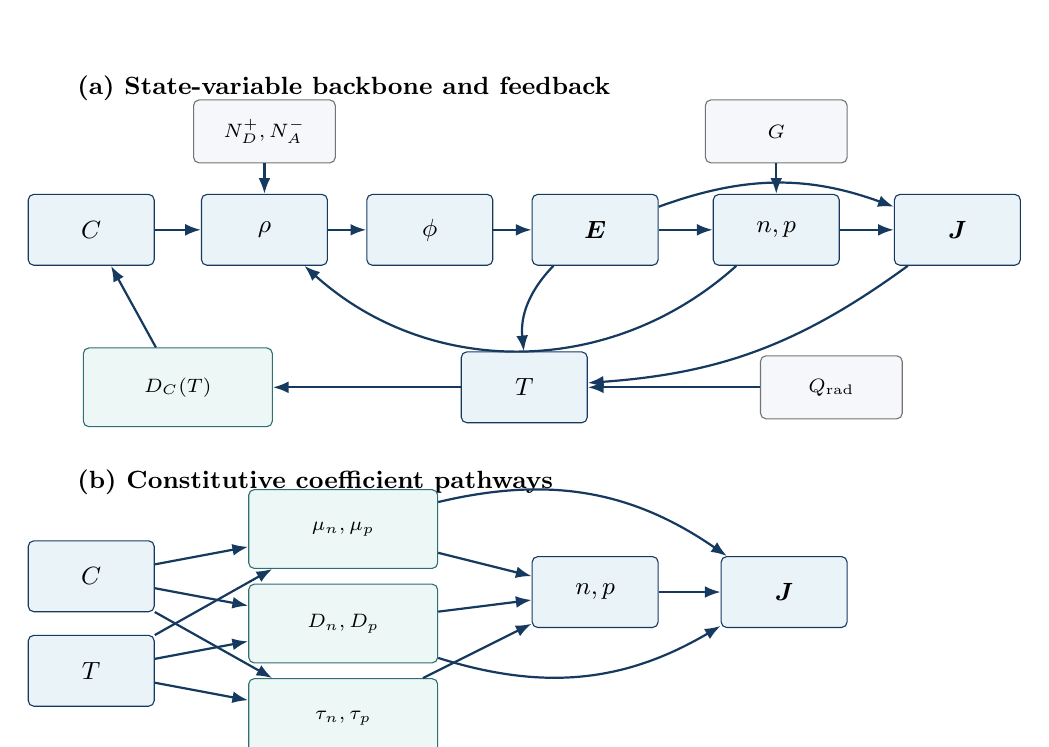
\begin{tikzpicture}[
field/.style={draw=TitleBlue,rounded corners=2pt,fill=SoftBlue,minimum width=16mm,minimum height=9mm,align=center,font=\small},
coef/.style={draw=AccentTeal,rounded corners=2pt,fill=SoftTeal,minimum width=24mm,minimum height=10mm,align=center,font=\scriptsize},
source/.style={draw=black!55,rounded corners=2pt,fill=SoftGray,minimum width=18mm,minimum height=8mm,align=center,font=\scriptsize},
arr/.style={-{Latex[length=2mm]},thick,draw=TitleBlue},
candidate/.style={-{Latex[length=2mm]},thick,dashed,draw=LearnedEdge}
]
% Panel A: state-variable backbone
\node[font=\small\bfseries,anchor=west] at (-0.3,1.8) {(a) State-variable backbone and feedback};
\node[field] (C) at (0,0) {$C$};
\node[field] (rho) at (2.2,0) {$\rho$};
\node[field] (phi) at (4.3,0) {$\phi$};
\node[field] (E) at (6.4,0) {$\Evec$};
\node[field] (np) at (8.7,0) {$n,p$};
\node[field] (J) at (11.0,0) {$\Jvec$};
\node[field] (T) at (5.5,-2.0) {$T$};
\node[coef] (DC) at (1.1,-2.0) {$D_C(T)$};
\node[source] (dop) at (2.2,1.25) {$N_D^+,N_A^-$};
\node[source] (G) at (8.7,1.25) {$G$};
\node[source] (Q) at (9.4,-2.0) {$Q_{\rm rad}$};
\draw[arr] (C) -- (rho);
\draw[arr] (dop) -- (rho);
\draw[arr] (rho) -- (phi);
\draw[arr] (phi) -- (E);
\draw[arr] (E) -- (np);
\draw[arr] (G) -- (np);
\draw[arr] (np) -- (J);
\draw[arr] (E) to[bend left=20] (J);
\draw[arr] (np) to[bend left=42] (rho);
\draw[arr] (J) to[bend left=16] (T);
\draw[arr] (E) to[bend right=25] (T);
\draw[arr] (Q) -- (T);
\draw[arr] (T) -- (DC);
\draw[arr] (DC) -- (C);

% Panel B: constitutive mediation
\begin{scope}[yshift=-4.4cm]
\node[font=\small\bfseries,anchor=west] at (-0.3,1.2) {(b) Constitutive coefficient pathways};
\node[field] (C2) at (0,0) {$C$};
\node[field] (T2) at (0,-1.2) {$T$};
\node[coef] (mu) at (3.2,0.6) {$\mu_n,\mu_p$};
\node[coef] (Dn) at (3.2,-0.6) {$D_n,D_p$};
\node[coef] (tau) at (3.2,-1.8) {$\tau_n,\tau_p$};
\node[field] (np2) at (6.4,-0.2) {$n,p$};
\node[field] (J2) at (8.8,-0.2) {$\Jvec$};
\draw[arr] (C2) -- (mu);
\draw[arr] (C2) -- (Dn);
\draw[arr] (C2) -- (tau);
\draw[arr] (T2) -- (mu);
\draw[arr] (T2) -- (Dn);
\draw[arr] (T2) -- (tau);
\draw[arr] (mu) -- (np2);
\draw[arr] (Dn) -- (np2);
\draw[arr] (tau) -- (np2);
\draw[arr] (mu) to[bend left=24] (J2);
\draw[arr] (Dn) to[bend right=24] (J2);
\draw[arr] (np2) -- (J2);
\end{scope}
\end{tikzpicture}}
\caption{Candidate physical dependency graph for the reduced Module 6 physics. Panel (a) shows the state-variable backbone, major feedback loops, and external sources. Panel (b) isolates the constitutive pathways through mobility, diffusivity, and lifetime. Solid arrows are direct dependencies in the reduced model. Candidate mechanisms such as charged-defect drift are retained in the edge table and synthetic graph-family design rather than superimposed on this backbone diagram.}
\label{fig:physical_dependency_graph}
\end{figure}

\subsection{Direct, indirect, and redundant edges}

Suppose a model predicts a strong edge \(C\rightarrow\phi\). This association may be statistically real, but it is not necessarily a direct physical edge because \(C\) enters \(\rho\), and \(\rho\) enters Poisson's equation. If both \(\rho\) and \(\phi\) are nodes, the preferred representation is
\begin{equation}
C\rightarrow\rho\rightarrow\phi.
\end{equation}
A direct shortcut \(C\rightarrow\phi\) should be penalized unless it captures an omitted mechanism. This motivates conditional prediction tests and sparsity penalties.

\subsection{Edge mechanism taxonomy}

Each edge should carry a type label:
\begin{enumerate}[leftmargin=1.6em]
    \item \textbf{algebraic composition}: variables combine into another variable, such as \((n,p,C_j)\rightarrow\rho\);
    \item \textbf{constraint}: a source determines an algebraic field, such as \(\rho\rightarrow\phi\);
    \item \textbf{derivative}: one field is a derivative of another, such as \(\phi\rightarrow\Evec\);
    \item \textbf{constitutive}: a state changes a material coefficient, such as \(T\rightarrow\mu_n\);
    \item \textbf{transport driving}: a field or coefficient controls a flux, such as \(\Evec\rightarrow\Jvec_n\);
    \item \textbf{dynamic source}: a source changes an evolving state, such as \(G\rightarrow n\);
    \item \textbf{reaction}: one population affects another through a reaction rate;
    \item \textbf{heating}: electrical or reaction quantities enter the thermal equation;
    \item \textbf{external forcing}: radiation, bias, or boundary conditions drive an internal variable.
\end{enumerate}
Typed edges make the graph more interpretable and reduce the burden on the neural network.

\section{Coupling sequences derived from a physical graph}

\subsection{Why a total ordering may not exist}

The graph includes feedback loops such as
\begin{equation}
(n,p)\rightarrow\rho\rightarrow\phi\rightarrow\Evec\rightarrow(n,p),
\end{equation}
and
\begin{equation}
T\rightarrow D_C\rightarrow C\rightarrow\mu_{n,p}\rightarrow\Jvec\rightarrow T.
\end{equation}
A directed cycle prevents a standard topological ordering. Forcing the graph into a DAG would erase real feedback or reverse an edge incorrectly.

\subsection{Time unrolling}

A physical feedback loop becomes acyclic when causes and responses are assigned to explicit time indices. A generic time-lagged edge is
\begin{equation}
X_i(t)\rightarrow X_j(t+\ell_{ij}\dt).
\end{equation}
For example,
\begin{align}
T(t)&\rightarrow D_C(t),\\
D_C(t)&\rightarrow C(t+\dt),\\
C(t+\dt)&\rightarrow\rho(t+\dt),\\
\rho(t+\dt)&\rightarrow\phi(t+\dt),\\
\phi(t+\dt)&\rightarrow\Evec(t+\dt).
\end{align}
Algebraic relations may have zero lag, while transport and reaction edges generally have nonzero physical response times.

\begin{figure}[H]
\centering
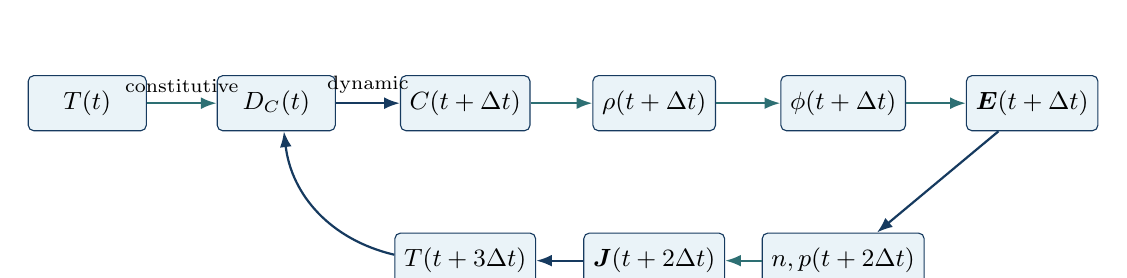
\begin{tikzpicture}[
node/.style={draw=TitleBlue,rounded corners=2pt,fill=SoftBlue,minimum width=15mm,minimum height=7mm,align=center,font=\small},
arr/.style={-{Latex[length=2mm]},thick,draw=TitleBlue},
zero/.style={-{Latex[length=2mm]},thick,draw=AccentTeal}
]
\node[node] (T0) at (0,0) {$T(t)$};
\node[node] (D0) at (2.4,0) {$D_C(t)$};
\node[node] (C1) at (4.8,0) {$C(t+\dt)$};
\node[node] (r1) at (7.2,0) {$\rho(t+\dt)$};
\node[node] (p1) at (9.6,0) {$\phi(t+\dt)$};
\node[node] (E1) at (12.0,0) {$\Evec(t+\dt)$};
\node[node] (n2) at (9.6,-2.0) {$n,p(t+2\dt)$};
\node[node] (J2) at (7.2,-2.0) {$\Jvec(t+2\dt)$};
\node[node] (T3) at (4.8,-2.0) {$T(t+3\dt)$};
\draw[zero] (T0) -- node[above,font=\scriptsize]{constitutive} (D0);
\draw[arr] (D0) -- node[above,font=\scriptsize]{dynamic} (C1);
\draw[zero] (C1) -- (r1);
\draw[zero] (r1) -- (p1);
\draw[zero] (p1) -- (E1);
\draw[arr] (E1) -- (n2);
\draw[zero] (n2) -- (J2);
\draw[arr] (J2) -- (T3);
\draw[arr] (T3) to[bend left=35] (D0);
\end{tikzpicture}
\caption{Illustrative time-unrolled physical dependency graph. Zero-lag algebraic or constitutive edges are shown separately from delayed dynamical edges. Time unrolling allows feedback without imposing an incorrect acyclicity assumption on the original physical system.}
\label{fig:time_unrolled_physical_graph}
\end{figure}

\subsection{Strongly connected components}

For a static directed graph, compute its strongly connected components. Every SCC is a maximal feedback group. Collapse each SCC into one supernode. The resulting condensation graph is always a DAG and can therefore be topologically ordered.

Let \(\mathcal{C}_1,\ldots,\mathcal{C}_K\) be the SCCs. The condensation graph is
\begin{equation}
\Gcal_{\mathrm{cond}}=(\{\mathcal{C}_k\},\Ecal_{\mathrm{cond}}).
\end{equation}
A physically admissible coupling sequence is then a topological ordering
\begin{equation}
\mathcal{C}_{\pi(1)}\prec\mathcal{C}_{\pi(2)}\prec\cdots\prec\mathcal{C}_{\pi(K)}.
\end{equation}
Variables within one SCC should be interpreted as a mutually coupled physical group rather than forcibly serialized.

\subsection{What the GNN should output}

The learned graph can therefore produce:
\begin{itemize}[leftmargin=1.5em]
    \item a directed edge list;
    \item edge mechanism types;
    \item edge strength as a function of state;
    \item zero-lag versus delayed classification;
    \item physical lag estimates;
    \item SCC feedback groups;
    \item a topological order of the SCC condensation graph;
    \item uncertainty for every item above.
\end{itemize}
This is the precise sense in which Module 11 attempts to find a coupling sequence.

\section{Graph fundamentals}

\subsection{Why graphs are the natural representation}

A graph is a collection of entities and relations:
\begin{equation}
\Gcal=(\Vcal,\Ecal).
\end{equation}
The node set \(\Vcal=\{v_1,\ldots,v_{N_v}\}\) contains physical quantities. A directed edge \((i,j)\in\Ecal\) means that information flows from source node \(i\) to target node \(j\). Each node has features \(\xvec_i\), and each edge can have features \(\evec_{ij}\).

Graphs are appropriate because the Module 11 variables are heterogeneous and relational. Temperature, defect concentration, electric field, carrier density, mobility, and radiation source do not form a simple image-like array. Their meaning lies partly in how they influence one another.

\subsection{Directed, undirected, homogeneous, and heterogeneous graphs}

An undirected graph treats \(i\leftrightarrow j\) symmetrically. That is generally unsuitable for physical dependency discovery because \(\rho\rightarrow\phi\) is not equivalent to \(\phi\rightarrow\rho\). The graph should be directed.

A homogeneous graph assigns the same semantic type to all nodes and edges. Module 11 is naturally heterogeneous: field nodes, coefficient nodes, source nodes, and reaction nodes have different meanings, while edge types distinguish constraints, constitutive laws, transport, reactions, and heating.

\subsection{Adjacency matrices}

For a directed weighted graph, define
\begin{equation}
A_{ij}=\begin{cases}
a_{ij}, & i\rightarrow j\text{ is present},\\0,&\text{otherwise.}\end{cases}
\end{equation}
The convention is source row \(i\), target column \(j\). Because conventions differ across software, every implementation must document this choice and test it on a two-node graph.

A binary adjacency matrix expresses topology. A weighted adjacency matrix expresses effective influence. A typed graph can use one adjacency matrix for each mechanism class:
\begin{equation}
\Amat=\sum_{r=1}^{R}\Amat^{(r)},
\end{equation}
where \(r\) indexes relation types.

\subsection{Permutation equivariance}

Node ordering is arbitrary. If a permutation matrix \(\bm{P}\) reorders node labels, the features and adjacency transform as
\begin{equation}
\Xmat' = \bm{P}\Xmat,\qquad
\Amat'=\bm{P}\Amat\bm{P}^{T}.
\end{equation}
A node-level GNN should be permutation equivariant:
\begin{equation}
f(\bm{P}\Xmat,\bm{P}\Amat\bm{P}^{T})=\bm{P}f(\Xmat,\Amat).
\end{equation}
This property prevents the network from assigning meaning to an arbitrary storage order.

\subsection{Receptive field and depth}

After one message-passing layer, a node receives information from its one-hop parents. After \(L\) layers, information can propagate across paths of length up to \(L\). The variable graph is small, so two to five message-passing layers are normally sufficient. Excessive depth can cause oversmoothing, in which node embeddings become indistinguishable.

\section{Neural-network foundations needed for GNNs}

\subsection{A neuron and a multilayer perceptron}

A dense neural layer computes
\begin{equation}
\hvec^{(\ell+1)}=\sigma\left(\Wmat^{(\ell)}\hvec^{(\ell)}+\bm{b}^{(\ell)}\right),
\end{equation}
where \(\sigma\) is a nonlinear activation. A multilayer perceptron composes several such layers. GNNs use MLPs inside edge-message and node-update functions, but they also respect graph structure through aggregation.

\subsection{Training as optimization}

Given samples \(\{(x_s,y_s)\}\), neural parameters are obtained by minimizing
\begin{equation}
\thetavec^*=\argmin_{\thetavec}\frac{1}{N}\sum_{s=1}^{N}\Lcal\left(f_{\thetavec}(x_s),y_s\right).
\end{equation}
For Module 11, \(x_s\) is a physical-variable graph plus trajectory context. Targets can include next-state variables, edge existence, edge type, edge lag, intervention response, and graph-level uncertainty.

\subsection{Normalization is physically essential}

The physical variables span many orders of magnitude. Defect concentrations, carrier densities, electric fields, mobilities, and heat sources cannot be passed to one network in raw SI units without severe conditioning problems. A positive variable \(x\) can be transformed as
\begin{equation}
\tilde{x}=\frac{\log(x+x_{\mathrm{floor}})-\mu_{\log x}}{\sigma_{\log x}}.
\end{equation}
Signed variables can use a signed logarithm,
\begin{equation}
\tilde{x}=\frac{\operatorname{sign}(x)\log(1+|x|/x_0)-\mu_x}{\sigma_x}.
\end{equation}
Normalization statistics must be computed from the training split only.

\subsection{Overfitting and leakage}

Data leakage occurs if different time steps from the same synthetic case are divided across train and test sets. The network can memorize case-specific parameters. Entire physical cases, source realizations, and intervention pairs must remain in one split. Regularization, early stopping, dropout, weight decay, graph sparsity, and independent topology tests should all be used.

\section{Message passing: the core GNN operation}

\subsection{General equations}

At layer \(\ell\), a directed message from node \(i\) to node \(j\) is
\begin{equation}
\mvec_{ij}^{(\ell)}
=\phi_m^{(\ell)}\left(
\hvec_i^{(\ell)},
\hvec_j^{(\ell)},
\evec_{ij},
\gvec
\right).
\label{eq:message}
\end{equation}
The target node aggregates incoming messages:
\begin{equation}
\bar{\mvec}_j^{(\ell)}
=\Agg_{i\in\mathcal{N}_{\mathrm{in}}(j)}\mvec_{ij}^{(\ell)}.
\label{eq:aggregation}
\end{equation}
The node then updates:
\begin{equation}
\hvec_j^{(\ell+1)}
=\phi_v^{(\ell)}\left(
\hvec_j^{(\ell)},
\bar{\mvec}_j^{(\ell)},
\gvec
\right).
\label{eq:node_update}
\end{equation}
The aggregation must be permutation invariant. Sum aggregation is expressive and preserves accumulated influence; mean aggregation removes degree dependence; maximum aggregation selects dominant mechanisms; attention learns normalized weights.

\subsection{Directed typed messages}

For relation type \(r\), use a relation-specific message function:
\begin{equation}
\mvec_{ij}^{(r)}=a_{ij}^{(r)}\phi_m^{(r)}\left(\hvec_i,\hvec_j,\evec_{ij},\gvec\right).
\end{equation}
A constraint edge should not be forced to use the same parameters as a heating edge. Relation-specific functions encode this distinction.

\subsection{Project-specific edge inference}

A practical directed edge logit is
\begin{equation}
\bm{\alpha}_{ij}
=\MLP_{\mathrm{edge}}\left[
\hvec_i,
\hvec_j,
\hvec_i-\hvec_j,
\hvec_i\odot\hvec_j,
\evec_{ij}^{\mathrm{prior}},
\gvec
\right].
\label{eq:edge_logits}
\end{equation}
The output can parameterize the probabilities
\begin{equation}
p(z_{ij}=r)=\softmax(\bm{\alpha}_{ij})_r,
\end{equation}
where \(r\in\{\text{none},\text{constraint},\text{constitutive},\text{dynamic},\text{reaction},\text{heating},\ldots\}\).

Direction is handled by evaluating \(i\rightarrow j\) and \(j\rightarrow i\) separately. Symmetrizing the logits would destroy directionality.

\subsection{Readout functions}

Node readouts predict future physical descriptors:
\begin{equation}
\widehat{\zvec}_j(t+\dt)=\Dec_j\left(\hvec_j^{(L)}\right).
\end{equation}
Edge readouts predict existence, type, strength, sign, and lag. Graph-level readouts can summarize uncertainty, number of SCCs, and whether the inferred graph is sufficiently supported by the data.

\begin{figure}[H]
\centering
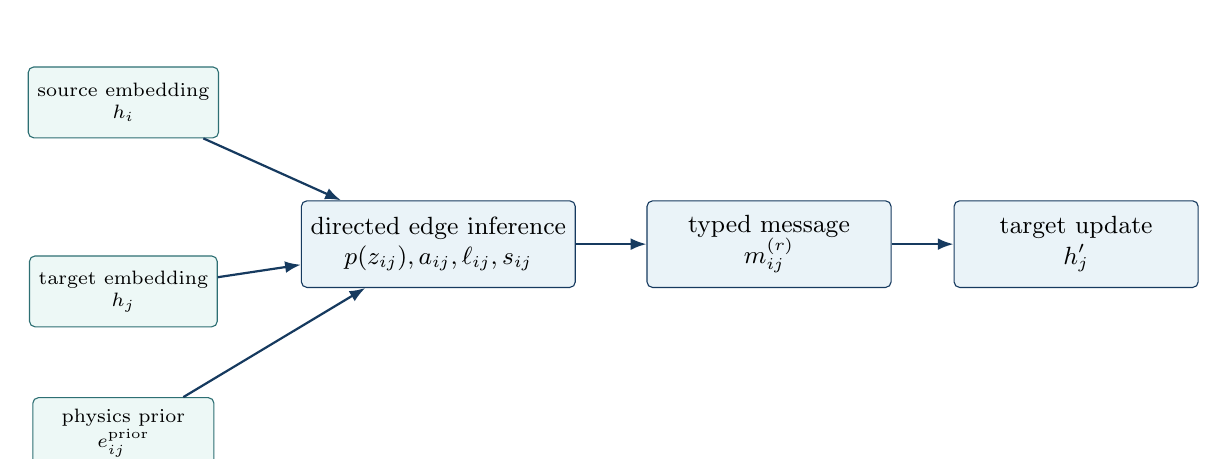
\begin{tikzpicture}[
box/.style={draw=TitleBlue,rounded corners=2pt,fill=SoftBlue,minimum width=31mm,minimum height=11mm,align=center,font=\small},
small/.style={draw=AccentTeal,rounded corners=2pt,fill=SoftTeal,minimum width=23mm,minimum height=9mm,align=center,font=\scriptsize},
arr/.style={-{Latex[length=2mm]},thick,draw=TitleBlue}
]
\node[small] (si) at (0,1.2) {source embedding\\$h_i$};
\node[small] (tj) at (0,-1.2) {target embedding\\$h_j$};
\node[small] (pr) at (0,-3.0) {physics prior\\$e_{ij}^{\rm prior}$};
\node[box] (edge) at (4.0,-0.6) {directed edge inference\\$p(z_{ij}),a_{ij},\ell_{ij},s_{ij}$};
\node[box] (msg) at (8.2,-0.6) {typed message\\$m_{ij}^{(r)}$};
\node[box] (agg) at (12.1,-0.6) {target update\\$h_j^{\prime}$};
\draw[arr] (si) -- (edge);
\draw[arr] (tj) -- (edge);
\draw[arr] (pr) -- (edge);
\draw[arr] (edge) -- (msg);
\draw[arr] (msg) -- (agg);
\end{tikzpicture}
\caption{Directed physical-edge inference and message passing. The model first estimates the relation from source to target, then uses that relation to form a typed message and update the target variable representation.}
\label{fig:edge_inference_block}
\end{figure}

\section{Major GNN architectures and their relevance}

\subsection{Graph convolutional networks}

A common GCN layer is
\begin{equation}
\Hmat^{(\ell+1)}
=\sigma\left(\widetilde{\Dmat}^{-1/2}\widetilde{\Amat}\widetilde{\Dmat}^{-1/2}\Hmat^{(\ell)}\Wmat^{(\ell)}\right),
\end{equation}
where \(\widetilde{\Amat}=\Amat+\Id\). GCNs are useful baselines, but the standard form assumes a fixed adjacency and often treats directions or relation types too simply for Module 11.

\subsection{GraphSAGE}

GraphSAGE computes
\begin{align}
\bar{\hvec}_j^{(\ell)}&=\Agg\{\hvec_i^{(\ell)}:i\in\mathcal{N}(j)\},\\
\hvec_j^{(\ell+1)}&=\sigma\left(\Wmat^{(\ell)}[\hvec_j^{(\ell)}\Vert\bar{\hvec}_j^{(\ell)}]\right).
\end{align}
Its inductive formulation can generalize to graphs containing additional defect species or coefficient nodes not seen in every training sample.

\subsection{Graph attention networks}

A GAT uses attention coefficients
\begin{equation}
\alpha_{ij}=\frac{\exp(e_{ij})}{\sum_{k\in\mathcal{N}(j)}\exp(e_{kj})}.
\end{equation}
Attention is useful for state-dependent edge strength, but attention weights are not automatically causal or physically identifiable. They must be tested by interventions and predictive ablations.

\subsection{Typed message-passing networks}

A relational or typed MPNN uses a separate transformation for each physical relation:
\begin{equation}
\bar{\mvec}_j=\sum_r\sum_{i\in\mathcal{N}_r(j)}\phi_m^{(r)}(\hvec_i,\hvec_j,\evec_{ij}).
\end{equation}
This is the recommended architecture family because it matches the heterogeneous edge taxonomy.

\subsection{Neural relational inference}

NRI uses an encoder to infer latent edge types from observed trajectories and a decoder to predict dynamics conditioned on the inferred graph. This matches the core Module 11 problem. Strong physical priors can restrict the candidate edge set and assign interpretable edge categories instead of anonymous relation labels.

\section{Temporal graphs and dynamical dependence}

\subsection{Instantaneous and lagged edges}

The graph should separate two classes:
\begin{align}
X_i(t)&\rightarrow X_j(t) &&\text{zero-lag algebraic or constitutive edge},\\
X_i(t)&\rightarrow X_j(t+\ell\dt) &&\text{lagged dynamical edge}.
\end{align}
A single static adjacency matrix loses this distinction. One solution is a family of lag matrices
\begin{equation}
\Amat^{(0)},\Amat^{(1)},\ldots,\Amat^{(L_{\max})}.
\end{equation}

\subsection{Recurrent graph model}

Let \(\zvec_i^n\) be the compressed state of variable \(i\) at time \(t_n\). A recurrent graph decoder can use
\begin{equation}
\zvec_j^{n+1}=F_j\left(\zvec_j^n,\sum_i\sum_{\ell=0}^{L_{\max}}A_{ij}^{(\ell)}M_{ij}^{(\ell)}(\zvec_i^{n-\ell},\zvec_j^n),\gvec^n\right).
\label{eq:temporal_graph_decoder}
\end{equation}
The model must use causal masking so that future data cannot influence the inferred past graph.

\subsection{State-dependent graph strength}

Topology may remain fixed while edge strength varies:
\begin{equation}
a_{ij}(t)=\sigmoid\left(g_{ij}(\hvec_i(t),\hvec_j(t),\gvec(t))\right).
\end{equation}
For example, Joule-heating feedback may be negligible at low bias and strong at high current. Defect-charge effects may be negligible before irradiation and dominant after damage accumulation. Learning state-dependent weights is therefore more realistic than learning one constant matrix.

\section{Learning graph structure}

\subsection{Fixed candidate graph, weighted graph, and latent graph}

Three levels are possible:
\begin{enumerate}[leftmargin=1.6em]
    \item \textbf{fixed topology}: all trusted edges are fixed and only strengths are learned;
    \item \textbf{candidate topology}: a physics-defined superset is given and the model gates edges on or off;
    \item \textbf{fully latent topology}: every directed pair is allowed.
\end{enumerate}
The second option is recommended. The first cannot discover omitted candidate mechanisms. The third permits too many spurious edges and requires far more data.

\subsection{Continuous edge gates}

A relaxed gate can be written
\begin{equation}
a_{ij}=\sigmoid(\alpha_{ij}).
\end{equation}
Sparsity is encouraged with
\begin{equation}
\Lsparse=\sum_{i\neq j}|a_{ij}|.
\end{equation}
A gate close to zero suppresses messages but remains differentiable.

\subsection{Discrete edge types}

For categorical edge types, Gumbel-softmax provides a differentiable approximation to a discrete sample:
\begin{equation}
\tilde{z}_{ij,r}=\frac{\exp((\log\pi_{ij,r}+g_r)/\tau_g)}{\sum_s\exp((\log\pi_{ij,s}+g_s)/\tau_g)}.
\end{equation}
The temperature \(\tau_g\) is gradually reduced during training. A hard edge assignment should be evaluated at test time.

\subsection{Causal discovery is not automatic}

Predictive association does not prove causation. Two variables can correlate because of a common driver. For example, \(C\) and \(T\) can both rise after a radiation pulse even if neither directly drives the other in a simplified generator. Directionality must be supported by temporal precedence, conditional prediction, interventions, and physical equations.

\subsection{Interventions}

An intervention changes one mechanism while holding the rest of the generator fixed. If defect-dependent mobility is disabled, the response difference isolates the path
\begin{equation}
C\rightarrow\mu_{n,p}\rightarrow\Jvec.
\end{equation}
Intervention pairs provide much stronger supervision than passive trajectories.

\section{Proposed Module 11 architecture}

\subsection{Node definition}

The first model should use approximately 15--30 variable nodes. A recommended reduced node set is
\begin{equation}
\{C,T,D_C,\rho,\phi,\Evec,n,p,\mu_n,\mu_p,D_n,D_p,\tau_n,\tau_p,\Jvec,G,Q_{\mathrm{rad}},Q_{\mathrm{J}}\}.
\end{equation}
A later model can separate defect species, electron and hole currents, reaction rates, and heat-source components.

\subsection{Field-to-node feature extraction}

Although many nodes represent spatial fields, the graph is not spatial. Each field is summarized by a feature vector such as
\begin{equation}
\xvec_i(t)=\left[
\overline{X_i},
\sigma(X_i),
\min X_i,
\max X_i,
\|X_i\|_2,
\|\nabla X_i\|_2,
q_{0.1},q_{0.5},q_{0.9},
\dot{\overline{X_i}},
a_{i,1},\ldots,a_{i,K}
\right],
\end{equation}
where \(a_{i,k}\) are optional POD coefficients. These descriptors preserve field information while keeping graph nodes tied to physical variables.

\subsection{Node-type encoder}

Different variable types require different encoders:
\begin{equation}
\hvec_i^0=\Enc_{\tau(i)}(\xvec_i),
\end{equation}
where \(\tau(i)\) denotes field, coefficient, source, or rate node. Type-specific encoders avoid asking one normalization and one MLP to handle incompatible semantics.

\subsection{Edge prior mask}

Define a candidate mask \(M_{ij}\in\{0,1\}\). The edge logit is
\begin{equation}
\alpha_{ij}\leftarrow
\begin{cases}
\alpha_{ij}, & M_{ij}=1,\\
-\infty, & M_{ij}=0.
\end{cases}
\end{equation}
Trusted impossible edges are excluded. Plausible but uncertain edges remain learnable. Candidate masks should be versioned because they encode scientific assumptions.

\subsection{Encoder-decoder structure}

The recommended model is:
\begin{enumerate}[leftmargin=1.6em]
    \item encode node trajectories over a context window;
    \item infer directed edge probabilities, types, signs, and lags;
    \item pass typed messages through the inferred graph;
    \item decode future node states;
    \item compute physics and intervention losses;
    \item derive SCCs and the condensation sequence from the thresholded graph.
\end{enumerate}

\subsection{Graph output and thresholding}

At inference time, report continuous probabilities first. A binary graph is obtained using a validation-selected threshold \(\tau_A\):
\begin{equation}
\widehat{A}_{ij}=\mathbb{I}\left[p(i\rightarrow j)>\tau_A\right].
\end{equation}
The threshold should maximize a balanced graph-recovery metric on validation data, not be chosen after inspecting the test set.

\section{Synthetic data: what it can and cannot establish}

\subsection{What synthetic data can prove}

Synthetic data are sufficient to test whether the method can recover a known graph, distinguish direct from indirect dependence, identify edge direction and type, estimate physical lags, track regime-dependent strengths, generalize to held-out parameter combinations, and predict the response to mechanism ablations.

\subsection{What synthetic data cannot prove}

The learned graph is only as complete as the generator family. If the simulator omits an interface trap mechanism, nonlocal phonon effect, field-assisted reaction, or material transition, the network cannot discover it from data that never contain it. Therefore,
\begin{equation}
\text{recovered graph}\approx\text{best graph inside the synthetic model family},
\end{equation}
not necessarily the complete graph of a real device.

\subsection{Avoiding circularity}

The graph labels must come from equations and explicit mechanism switches, not from the hand-drawn Module 6 diagram alone. The simulator should expose every candidate edge through a coupling coefficient or mechanism flag. Synthetic cases should include multiple graph topologies, not one fixed topology repeated under different parameters. Otherwise, the network can memorize the graph without learning how evidence supports it.

\section{Synthetic sample definition}

One synthetic sample should contain
\begin{equation}
\mathcal{D}^{(s)}=
\left
\{
\mathcal{P}^{(s)},
\mathcal{B}^{(s)},
\mathcal{I}^{(s)},
\mathcal{S}^{(s)},
\mathcal{K}^{(s)},
\mathcal{X}^{(s)}(t),
\mathcal{Y}^{(s)}(t),
\Amat_{\mathrm{true}}^{(s)},
\bm{Z}_{\mathrm{true}}^{(s)},
\bm{L}_{\mathrm{true}}^{(s)}
\right\}.
\label{eq:synthetic_sample}
\end{equation}
Here:
\begin{itemize}[leftmargin=1.5em]
    \item \(\mathcal{P}\) contains physical parameters;
    \item \(\mathcal{B}\) contains boundary and forcing conditions;
    \item \(\mathcal{I}\) contains initial conditions;
    \item \(\mathcal{S}\) contains source realizations;
    \item \(\mathcal{K}\) contains active mechanism switches and edge multipliers;
    \item \(\mathcal{X}(t)\) contains raw field trajectories;
    \item \(\mathcal{Y}(t)\) contains normalized variable-node features;
    \item \(\Amat_{\mathrm{true}}\) is the known directed graph;
    \item \(\bm{Z}_{\mathrm{true}}\) stores edge types and signs;
    \item \(\bm{L}_{\mathrm{true}}\) stores physical lags or lag classes.
\end{itemize}

\section{Synthetic generator architecture}

\subsection{Layer 1: graph-family sampler}

Begin with a trusted core graph and a set of switchable candidate edges. For each sample, draw mechanism switches
\begin{equation}
k_e\in\{0,1\}
\end{equation}
or continuous edge multipliers
\begin{equation}
\gamma_e\in[0,1].
\end{equation}
Examples include:
\begin{align}
\gamma_{C\rightarrow\rho}&: \text{effective defect charge},\\
\gamma_{C\rightarrow\mu}&: \text{defect mobility degradation},\\
\gamma_{C\rightarrow\tau}&: \text{defect-assisted recombination},\\
\gamma_{\Evec\rightarrow C}&: \text{charged-defect drift},\\
\gamma_{\Jvec,\Evec\rightarrow T}&: \text{Joule heating},\\
\gamma_{R\rightarrow T}&: \text{recombination heating},\\
\gamma_{T\rightarrow R_j}&: \text{thermally activated defect reactions}.
\end{align}
The ground-truth adjacency is generated directly from active switches.

\subsection{Layer 2: parameter sampler}

Parameters should be sampled jointly rather than one at a time. Use a mixture of:
\begin{itemize}[leftmargin=1.5em]
    \item uniform sampling for bounded approximately linear uncertainty;
    \item log-uniform sampling for positive quantities spanning orders of magnitude;
    \item beta distributions for values concentrated near a nominal range;
    \item categorical sampling for material, boundary, or mechanism families;
    \item Latin hypercube or Sobol designs for efficient multidimensional coverage;
    \item targeted stress samples near known transitions or stiffness boundaries.
\end{itemize}

\begin{figure}[H]
\centering
\includegraphics[width=0.88\textwidth]{figures/module11/module11_sampling_priors.pdf}
\caption{Illustrative sampling priors. Uniform, log-uniform, and beta distributions serve different purposes. The plotted curves are conceptual and not calibrated project distributions.}
\label{fig:sampling_priors}
\end{figure}

\subsection{Layer 3: source and initial-condition sampler}

Radiation-induced defect and heat sources should vary in amplitude, location, width, shape, and temporal profile. A Gaussian source is
\begin{equation}
S_C(x,y,t)=A_C
\exp\left[-\frac{(x-x_0)^2}{2\sigma_x^2}-\frac{(y-y_0)^2}{2\sigma_y^2}\right]f_C(t).
\label{eq:gaussian_defect_source}
\end{equation}
Useful temporal functions include:
\begin{align}
f_{\mathrm{imp}}(t)&\approx \exp[-(t-t_0)^2/(2\sigma_t^2)],\\
f_{\mathrm{step}}(t)&=H(t-t_0),\\
f_{\mathrm{decay}}(t)&=H(t-t_0)e^{-(t-t_0)/\tau_s},\\
f_{\mathrm{pulse}}(t)&=H(t-t_0)-H(t-t_1).
\end{align}

A smooth random field can be created through a truncated Karhunen--Lo\`eve expansion:
\begin{equation}
X(x,y)=\bar{X}(x,y)+\sum_{k=1}^{K}\sqrt{\lambda_k}\xi_k\psi_k(x,y),
\qquad \xi_k\sim\mathcal{N}(0,1).
\label{eq:kl_random_field}
\end{equation}
This varies field morphology without changing the graph topology.

\subsection{Layer 4: mechanistic trajectory generator}

Run the coupled physics equations with the sampled graph, parameters, sources, and initial conditions. The generator must save raw states at every requested physical time. The numerical method is not a target; only the resulting trajectories and residuals are used.

\subsection{Layer 5: intervention generator}

For a selected baseline sample, create matched counterfactuals by changing one mechanism:
\begin{equation}
\left(\mathcal{P},\mathcal{B},\mathcal{I},\mathcal{S}\right)_{\mathrm{baseline}}
=
\left(\mathcal{P},\mathcal{B},\mathcal{I},\mathcal{S}\right)_{\mathrm{intervention}},
\end{equation}
while \(k_e\) or \(\gamma_e\) changes. The matched design isolates the edge effect.

\subsection{Layer 6: observation and noise model}

Create several observation levels:
\begin{enumerate}[leftmargin=1.6em]
    \item exact simulator fields;
    \item field summaries with no added noise;
    \item multiplicative and additive noise;
    \item missing variables at selected times;
    \item coarser temporal sampling;
    \item model-discrepancy cases generated by a richer equation set.
\end{enumerate}
For positive quantities, multiplicative noise is natural:
\begin{equation}
X_{\mathrm{obs}}=X\exp(\sigma_\eta\eta),\qquad \eta\sim\mathcal{N}(0,1).
\end{equation}
For signed quantities, use additive noise scaled by a robust range.

\section{Recommended synthetic parameter ranges}

The following ranges are initial stress-test ranges, not calibrated device specifications. They should be narrowed when material-specific data become available.

\small
\begin{longtable}{p{0.20\textwidth}p{0.18\textwidth}p{0.15\textwidth}p{0.27\textwidth}}
\toprule
\textbf{Quantity} & \textbf{Illustrative range} & \textbf{Distribution} & \textbf{Purpose} \\
\midrule
\endfirsthead
\toprule
\textbf{Quantity} & \textbf{Illustrative range} & \textbf{Distribution} & \textbf{Purpose} \\
\midrule
\endhead
Ambient temperature \(T_0\) & \(250\)--\(400\,\mathrm{K}\) & uniform or beta & Baseline thermal state and coefficient variation. \\
Transient temperature rise & \(10^{-3}\)--\(10^{2}\,\mathrm{K}\) & log-uniform & Weak to strong heating. \\
Applied bias magnitude & \(10^{-3}\)--\(10^{2}\,\mathrm{V}\) & signed log-uniform & Carrier-electrostatic feedback strength. \\
Peak effective defect density \(C_{\max}\) & \(10^{14}\)--\(10^{24}\,\mathrm{m^{-3}}\) & log-uniform & Pristine to heavily damaged regimes. \\
Defect charge magnitude \(|z_{\mathrm{def}}|\) & \(0\)--2 & categorical or continuous & Activates or weakens \(C\rightarrow\rho\). \\
Defect source amplitude \(A_C\) & problem-scaled over 6--10 decades & log-uniform & Radiation-damage intensity. \\
Defect diffusivity prefactor \(D_{0,C}\) & \(10^{-20}\)--\(10^{-4}\,\mathrm{m^2/s}\) & log-uniform & Frozen to mobile defects. \\
Defect activation energy \(E_a\) & \(0.05\)--\(2.0\,\mathrm{eV}\) & uniform/beta & Thermal sensitivity of defect motion and reaction. \\
Annealing time scale & \(10^{-9}\)--\(10^{8}\,\mathrm{s}\) & log-uniform & Fast recovery to long-term damage. \\
Electron mobility \(\mu_{n,0}\) & \(10^{-4}\)--\(1\,\mathrm{m^2/(V\,s)}\) & log-uniform & Carrier drift strength. \\
Hole mobility \(\mu_{p,0}\) & \(10^{-5}\)--\(0.5\,\mathrm{m^2/(V\,s)}\) & log-uniform & Hole drift strength. \\
Mobility temperature exponent & \(0\)--3 & uniform & Controls \(T\rightarrow\mu\). \\
Defect mobility-degradation factor & \(0\)--\(10^{3}\) normalized & log-uniform plus zero mass & Controls \(C\rightarrow\mu\). \\
Carrier lifetime \(\tau_n,\tau_p\) & \(10^{-12}\)--\(10^{-2}\,\mathrm{s}\) & log-uniform & Recombination time scales. \\
Carrier generation \(G\) & problem-scaled over 8 decades & log-uniform plus zero mass & Radiation or external carrier source. \\
Thermal conductivity \(k\) & \(0.1\)--\(500\,\mathrm{W/(m\,K)}\) & log-uniform & Heat-removal strength. \\
Volumetric heat capacity \(\rho_m c_p\) & \(10^{4}\)--\(10^{7}\,\mathrm{J/(m^3\,K)}\) & log-uniform & Thermal response time. \\
Radiation heat source \(Q_{\mathrm{rad}}\) & problem-scaled over 10 decades & log-uniform plus zero mass & Direct thermal forcing. \\
Joule-heating multiplier \(\gamma_J\) & \(0\)--1.5 & mixture with mass at zero and one & Edge activation and model mismatch. \\
Recombination-heating multiplier & \(0\)--1.5 & mixture & Tests additional heat pathway. \\
Edge lag class \(\ell_{ij}\) & \(0\)--8 stored time steps & categorical & Lag recovery. \\
Observation noise & 0--10\% RMS & mixture & Robustness and uncertainty calibration. \\
\bottomrule
\end{longtable}
\normalsize

\subsection{Correlated sampling}

Some parameters should not be independent. Examples include the Einstein relation
\begin{equation}
D_n=\frac{k_BT}{q}\mu_n,\qquad D_p=\frac{k_BT}{q}\mu_p,
\end{equation}
and Arrhenius diffusivity
\begin{equation}
D_C(T)=D_{0,C}\exp\left(-\frac{E_a}{k_BT}\right).
\end{equation}
Sample the independent base parameters, then compute dependent coefficients. Violating such relations without labeling the case as a discrepancy study teaches the GNN physically impossible combinations.

\subsection{Dimensionless regime sampling}

Raw parameter ranges do not guarantee coverage of physically distinct regimes. Stratify samples using dimensionless groups such as
\begin{align}
\Pe_n&=\frac{\mu_n |\Evec|L}{D_n},\\
\Da_C&=\frac{L^2}{D_C\tau_{\mathrm{react}}},\\
\Gamma_J&=\frac{Q_JL^2}{k\Delta T_{\mathrm{ref}}},\\
\Gamma_\rho&=\frac{q|z|C L^2}{\epsilon\Delta\phi_{\mathrm{ref}}}.
\end{align}
Balanced coverage of low, intermediate, and high values helps the network observe when edges become weak or dominant.

\section{Detailed intervention library}

\subsection{Hard edge removal}

Set the mechanism coefficient exactly to zero. Examples are
\begin{align}
z_{\mathrm{def}}&=0 &&\Rightarrow C\not\rightarrow\rho,\\
\alpha_{\mu C}&=0 &&\Rightarrow C\not\rightarrow\mu_{n,p},\\
\alpha_{\tau C}&=0 &&\Rightarrow C\not\rightarrow\tau_{n,p},\\
\gamma_J&=0 &&\Rightarrow (\Jvec,\Evec)\not\rightarrow T,\\
\mu_C&=0 &&\Rightarrow \Evec\not\rightarrow C \text{ through charged-defect drift}.
\end{align}

\subsection{Soft intervention}

Scale an edge by \(\gamma_e\in\{0.1,0.25,0.5,0.75,1.0,1.5\}\). A correct model should infer a monotonic increase in effective edge strength when the underlying mechanism is monotonic.

\subsection{Node intervention}

Clamp a variable to a prescribed trajectory:
\begin{equation}
\operatorname{do}\left(T(t)=T_{\mathrm{clamp}}(t)\right).
\end{equation}
This breaks incoming edges to \(T\) while preserving outgoing temperature effects. Node interventions help distinguish incoming from outgoing causation.

\subsection{Source intervention}

Apply isolated forcing to one source at a time: defect-only, carrier-only, heat-only, or bias-only excitation. Independent excitation improves graph identifiability because variables no longer move together solely due to one common radiation pulse.

\subsection{Factorial intervention design}

Single-edge ablations do not reveal interactions between mechanisms. A fractional factorial design over key switches can test whether two pathways mask or amplify each other. At minimum, include combinations of defect charge, defect-mobility degradation, defect-assisted recombination, and Joule heating.

\begin{figure}[H]
\centering
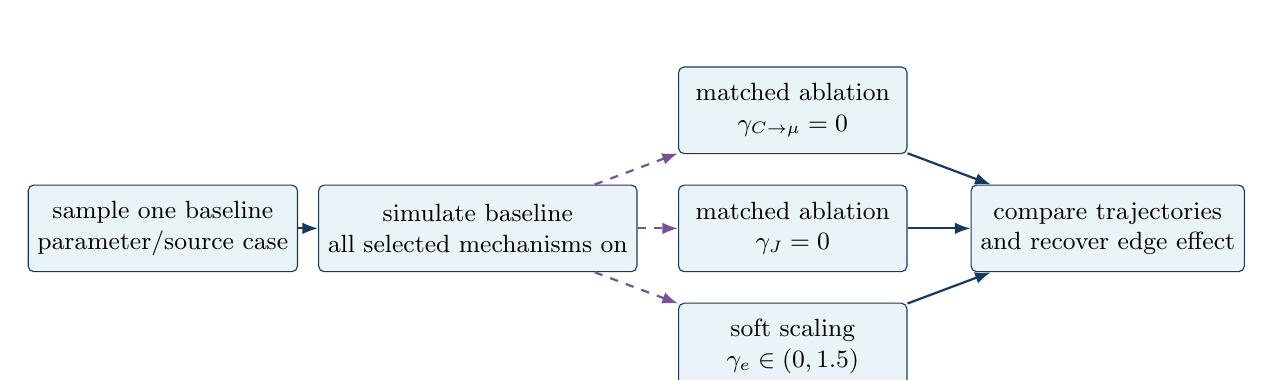
\begin{tikzpicture}[
box/.style={draw=TitleBlue,rounded corners=2pt,fill=SoftBlue,minimum width=29mm,minimum height=11mm,align=center,font=\small},
arr/.style={-{Latex[length=2mm]},thick,draw=TitleBlue},
branch/.style={-{Latex[length=2mm]},thick,dashed,draw=LearnedEdge}
]
\node[box] (base) at (0,0) {sample one baseline\\parameter/source case};
\node[box] (sim) at (4.0,0) {simulate baseline\\all selected mechanisms on};
\node[box] (abl1) at (8.0,1.5) {matched ablation\\$\gamma_{C\to\mu}=0$};
\node[box] (abl2) at (8.0,0) {matched ablation\\$\gamma_J=0$};
\node[box] (soft) at (8.0,-1.5) {soft scaling\\$\gamma_e\in(0,1.5)$};
\node[box] (diff) at (12.0,0) {compare trajectories\\and recover edge effect};
\draw[arr] (base) -- (sim);
\draw[branch] (sim) -- (abl1);
\draw[branch] (sim) -- (abl2);
\draw[branch] (sim) -- (soft);
\draw[arr] (abl1) -- (diff);
\draw[arr] (abl2) -- (diff);
\draw[arr] (soft) -- (diff);
\end{tikzpicture}
\caption{Matched intervention generation. The baseline and counterfactuals share parameters, sources, and initial conditions; only one physical mechanism changes.}
\label{fig:intervention_pipeline}
\end{figure}

\section{Synthetic dataset generation algorithm}

\begin{designbox}
\textbf{Algorithm: generate one graph-labeled synthetic family}
\begin{enumerate}[leftmargin=1.6em]
    \item Draw a graph family by activating the trusted core edges and sampling candidate mechanism switches.
    \item Draw independent base parameters using a stratified design.
    \item Enforce constitutive and dimensional constraints to obtain dependent coefficients.
    \item Draw radiation sources, bias, boundary conditions, and initial fields.
    \item Integrate the physical equations and save all variables at requested times.
    \item Compute raw and normalized node features.
    \item Store the exact directed adjacency, edge types, signs, lags, and mechanism multipliers.
    \item Generate matched hard and soft interventions for selected edges.
    \item Compute equation residuals and conservation diagnostics.
    \item Reject only numerically invalid cases using predeclared criteria; do not remove physically difficult cases simply because they are inconvenient.
\end{enumerate}
\end{designbox}

\subsection{Pseudocode}

\begin{lstlisting}[basicstyle=\ttfamily\small,frame=single,breaklines=true]
for graph_family = 1:N_graph_families
    mechanism = sample_mechanism_switches(candidate_edges);
    A_true, edge_type, edge_lag = build_ground_truth_graph(mechanism);

    for case_id = 1:N_cases_per_family
        base = sample_independent_parameters(design);
        params = enforce_physical_constraints(base, mechanism);
        source = sample_radiation_and_bias_sources(params);
        initial = sample_initial_conditions(params, source);

        trajectory = simulate_physical_case(params, source, initial, mechanism);
        features = extract_variable_node_features(trajectory);
        diagnostics = compute_physics_residuals(trajectory, params);

        save_case(features, trajectory, diagnostics,
                  A_true, edge_type, edge_lag, mechanism);

        for intervention = selected_interventions(mechanism)
            counterfactual = simulate_matched_intervention(
                params, source, initial, mechanism, intervention);
            save_intervention_pair(trajectory, counterfactual, intervention);
        end
    end
end
\end{lstlisting}

\subsection{Dataset size ladder}

A practical progression is:
\begin{enumerate}[leftmargin=1.6em]
    \item 100--300 toy ODE cases for debugging direction and lag;
    \item 500--2,000 lumped multiphysics cases for architecture selection;
    \item 2,000--10,000 reduced field-simulation cases for proof of concept;
    \item a smaller high-fidelity discrepancy set for robustness testing.
\end{enumerate}
Each baseline case can produce several intervention pairs, substantially increasing causal supervision.

\subsection{Active sampling}

After an initial model is trained, add cases where edge entropy is high:
\begin{equation}
H_{ij}=-\sum_r p(z_{ij}=r)\log p(z_{ij}=r).
\end{equation}
Also target physical regimes in which two candidate graphs make similar passive predictions but different intervention predictions.

\section{Training targets and losses}

\subsection{Multi-task objective}

A recommended objective is
\begin{equation}
\Lcal_{\mathrm{total}}
=\lambda_x\Lstate
+\lambda_e\Ledge
+\lambda_t\Ltype
+\lambda_{\ell}\Llag
+\lambda_p\Lphysics
+\lambda_c\Lcons
+\lambda_i\Lint
+\lambda_s\Lsparse
+\lambda_r\Lprior.
\label{eq:total_loss}
\end{equation}

\subsection{State-prediction loss}

For normalized node states,
\begin{equation}
\Lstate=\frac{1}{N_tN_v}\sum_{n,j}\left\|\widehat{\zvec}_j^{n+1}-\zvec_j^{n+1}\right\|_2^2.
\end{equation}
Multi-step rollout loss should also be included:
\begin{equation}
\Lstate^{(K)}=\sum_{k=1}^{K}w_k\left\|\widehat{\zvec}^{n+k}-\zvec^{n+k}\right\|_2^2.
\end{equation}
A graph that predicts only one step but drifts rapidly is not sufficient.

\subsection{Edge-existence loss}

For binary edge labels,
\begin{equation}
\Ledge=-\sum_{i\neq j}\left[y_{ij}\log p_{ij}+(1-y_{ij})\log(1-p_{ij})\right].
\end{equation}
Because absent edges outnumber present edges, use class weighting or focal loss.

\subsection{Edge-type and direction loss}

For relation type \(r\),
\begin{equation}
\Ltype=-\sum_{i\neq j}\sum_r y_{ijr}\log p_{ijr}.
\end{equation}
Direction is assessed through separate ordered pairs. A prediction of \(j\rightarrow i\) does not partially satisfy a true edge \(i\rightarrow j\).

\subsection{Lag loss}

For categorical lag classes,
\begin{equation}
\Llag=-\sum_{i,j,\ell}y_{ij\ell}\log p_{ij\ell}.
\end{equation}
For continuous delay estimates, use a robust regression loss such as Huber loss.

\subsection{Physics residual losses}

Predicted trajectories should satisfy reduced governing relations. Examples include
\begin{align}
\Rcal_{\rho}&=\rho-q\left[p-n+N_D^+-N_A^-+\sum_jz_jC_j\right],\\
\Rcal_{\phi}&=-\nabla\cdot(\epsilon\nabla\phi)-\rho,\\
\Rcal_E&=\Evec+\nabla\phi,\\
\Rcal_{J_n}&=\Jvec_n-q\mu_n n\Evec-qD_n\nabla n,\\
\Rcal_T&=\rho_mc_p\partial_tT-\nabla\cdot(k\nabla T)-Q_{\mathrm{tot}}.
\end{align}
Then
\begin{equation}
\Lphysics=\sum_q w_q\frac{\|\Rcal_q\|_2^2}{s_q^2+\eps}.
\end{equation}
The scales \(s_q\) prevent one equation from dominating solely because of units.

\subsection{Conservation losses}

Integrated carrier consistency can be enforced through
\begin{equation}
\frac{d}{dt}\int_\Omega n\,d\Omega
-\int_\Omega(G-R)\,d\Omega
-\frac{1}{q}\int_{\partial\Omega}\Jvec_n\cdot\hat{\bm n}\,d\Gamma=0,
\end{equation}
with analogous hole, defect, and energy balances.

\subsection{Intervention consistency}

For a matched baseline and intervention,
\begin{equation}
\Delta\zvec^{\mathrm{true}}=\zvec^{\mathrm{int}}-\zvec^{\mathrm{base}},
\end{equation}
require
\begin{equation}
\Lint=\left\|\Delta\widehat{\zvec}-\Delta\zvec^{\mathrm{true}}\right\|_2^2.
\end{equation}
This loss directly trains the model to predict mechanism-specific effects.

\subsection{Prior consistency and forbidden edges}

Hard-impossible edges are masked. Trusted edges can receive a soft prior:
\begin{equation}
\Lprior=\sum_{(i,j)\in\Ecal_{\mathrm{trusted}}}(1-p_{ij})^2
+\sum_{(i,j)\in\Ecal_{\mathrm{unlikely}}}\eta_{ij}p_{ij}^2.
\end{equation}
A soft prior allows the model to expose simulator inconsistencies rather than forcing agreement at all costs.

\subsection{Loss-weight selection}

Losses should be normalized, monitored separately, and tuned using validation performance. A curriculum can first train state prediction with a fixed graph, then activate edge learning, then add intervention and sparsity losses. Dynamically balancing gradients is preferable to arbitrary weights spanning many orders of magnitude.

\begin{figure}[H]
\centering
\includegraphics[width=0.84\textwidth]{figures/module11/module11_learning_curves.pdf}
\caption{Illustrative multi-term training behavior. These curves are conceptual and do not represent a trained Module 11 model. In the revised scope, the validation rollout loss measures physical-trajectory prediction rather than numerical schedule quality.}
\label{fig:learning_curves}
\end{figure}

\section{Training curriculum}

\subsection{Phase 0: analytic two- and three-node systems}

Verify edge orientation, lag handling, and intervention logic on systems with exact solutions. Examples include a chain \(x\rightarrow y\rightarrow z\), a common-cause structure \(x\leftarrow u\rightarrow y\), and a two-node delayed feedback loop.

\subsection{Phase 1: fixed graph, state prediction}

Provide the true adjacency and train only the dynamics decoder. Failure here indicates inadequate node features or model capacity, not graph-inference failure.

\subsection{Phase 2: edge strength}

Keep topology fixed but learn continuous mechanism multipliers. Verify that predicted strength tracks known \(\gamma_e\).

\subsection{Phase 3: edge presence and type}

Allow switchable candidate edges. Train on multiple graph families and evaluate exact topology recovery.

\subsection{Phase 4: lag and feedback groups}

Add time-lag classification and SCC analysis. Verify the condensation sequence against the known graph.

\subsection{Phase 5: noisy and discrepant data}

Add noise, missing variables, coarser time sampling, and richer hidden physics. The objective is calibrated uncertainty, not forced confident recovery.

\section{Train, validation, test, and OOD splits}

\subsection{Split by complete physical family}

All time steps, interventions, and source variants associated with one base case should remain in one split. Otherwise, nearly identical counterfactuals leak into training and test data.

\subsection{Topology split}

Hold out selected combinations of active candidate edges. This tests whether the model composes known mechanisms rather than memorizing complete graphs.

\subsection{Parameter extrapolation}

Reserve high-damage, high-bias, or extreme-temperature ranges for OOD testing. Report exactly which dimensions are outside the training support.

\subsection{Mechanism OOD}

Generate a test set containing an unmodeled pathway, such as recombination heating, while excluding that edge from the candidate graph. A reliable model should show elevated residuals or uncertainty rather than silently misattribute the effect.

\subsection{Source-shape transfer}

Train on Gaussian and rectangular source profiles and test on clustered or multi-spot sources. The graph should remain stable even when field morphology changes.

\section{Evaluation metrics}

\subsection{Graph topology}

Report directed edge precision, recall, and F1 score:
\begin{align}
\mathrm{Precision}&=\frac{TP}{TP+FP},\\
\mathrm{Recall}&=\frac{TP}{TP+FN},\\
F_1&=\frac{2\,\mathrm{Precision}\,\mathrm{Recall}}{\mathrm{Precision}+\mathrm{Recall}}.
\end{align}
Also report structural Hamming distance, AUROC, and area under the precision-recall curve.

\subsection{Direction and type}

Conditioned on a detected adjacency, report direction accuracy and edge-type accuracy. A reversed edge should count as a structural error even if the unordered pair is correct.

\subsection{Lag}

Report lag-class accuracy, mean absolute lag error, and uncertainty calibration. Zero-lag algebraic edges should be assessed separately from delayed dynamic edges.

\subsection{Edge strength}

For known continuous mechanism multipliers, report correlation, mean absolute error, and monotonicity violations between \(\gamma_e\) and predicted \(a_{ij}\).

\subsection{Trajectory and intervention prediction}

Report normalized one-step error, rollout error, intervention-effect error, and residual norms. A graph with good F1 but poor counterfactual prediction is not physically useful.

\subsection{SCC and sequence recovery}

Compare the inferred SCC partition with the true partition using adjusted Rand index or pairwise agreement. Compare the condensation-graph partial order rather than forcing an arbitrary order within feedback groups.

\subsection{Calibration}

For predicted edge probability \(p\), empirical correctness should be approximately \(p\). Reliability diagrams, expected calibration error, and Brier scores should be reported.

\begin{figure}[H]
\centering
\includegraphics[width=0.76\textwidth]{figures/module11/module11_edge_strength_heatmap.pdf}
\caption{Illustrative directed coupling-strength matrix. Rows are source variables and columns are targets. The values are conceptual and should not be interpreted as project results.}
\label{fig:edge_heatmap}
\end{figure}

\section{Baselines the GNN must beat}

A GNN should be compared against simpler structure-learning methods:
\begin{itemize}[leftmargin=1.5em]
    \item pairwise correlation and lagged cross-correlation;
    \item partial correlation conditioned on candidate mediators;
    \item linear vector autoregression and Granger-style tests;
    \item sparse regression on candidate nonlinear library terms;
    \item an MLP over concatenated variable features with pairwise edge heads;
    \item fixed hand-coded graph with learned edge strengths;
    \item neural relational inference without physics losses;
    \item ablations without intervention data or without relation types.
\end{itemize}
The strongest physics baseline is direct extraction from the known synthetic equations. The learned model is justified when it recovers that graph from observations and generalizes across graph families and regimes.

\section{Proof-of-concept experiment ladder}

\subsection{Experiment 0: three-node chain}

Use
\begin{align}
\dot{x}&=-a x+u(t),\\
\dot{y}&=-b y+c x,\\
\dot{z}&=-d z+e y.
\end{align}
The graph is \(x\rightarrow y\rightarrow z\). Verify that the model does not create a direct \(x\rightarrow z\) edge when \(y\) is observed.

\subsection{Experiment 1: common cause}

Use
\begin{align}
\dot{x}&=-a x+c u,\\
\dot{y}&=-b y+d u.
\end{align}
Passive trajectories correlate \(x\) and \(y\), but the true graph is \(u\rightarrow x\) and \(u\rightarrow y\). This tests resistance to spurious association.

\subsection{Experiment 2: delayed feedback}

Use
\begin{align}
\dot{x}(t)&=-a x(t)+b y(t-\tau_y),\\
\dot{y}(t)&=-c y(t)+d x(t-\tau_x).
\end{align}
Verify direction, lag, SCC recovery, and time-unrolled representation.

\subsection{Experiment 3: lumped Module 2--5 model}

Replace spatial derivatives by low-order effective terms and retain variables \(C,T,\rho,\phi,E,n,p,J\). Randomly activate graph mechanisms and generate thousands of inexpensive trajectories. This is the main architecture-selection environment.

\subsection{Experiment 4: reduced field simulation}

Generate field trajectories from the existing coupled physics modules, compress each physical field into variable-node descriptors, and recover the known graph. The graph topology remains variable based; no spatial adjacency is learned.

\subsection{Experiment 5: hidden-mechanism discrepancy}

Generate test trajectories with one pathway omitted from the candidate graph. Evaluate whether residuals and uncertainty identify inadequacy.

\section{Uncertainty and safe interpretation}

\subsection{Sources of uncertainty}

Uncertainty arises from finite data, overlapping effects, insufficient excitation, observation noise, hidden variables, model discrepancy, and neural optimization variability.

\subsection{Practical methods}

Use deep ensembles, Monte Carlo dropout, bootstrap resampling by physical case, and Bayesian or Dirichlet edge heads. Report edge probabilities and confidence intervals rather than only a thresholded graph.

\subsection{Abstention}

When the model is uncertain, it should return an unresolved edge or a set of plausible graphs. Scientific structure learning is harmed by mandatory hard decisions.

\section{Interpretability}

\subsection{Edge probability is not enough}

For every inferred edge, report supporting evidence:
\begin{itemize}[leftmargin=1.5em]
    \item trajectory prediction improvement when the edge is included;
    \item degradation when the edge is ablated;
    \item intervention response agreement;
    \item physical residual reduction;
    \item edge probability across ensemble members;
    \item state regimes where the edge becomes strong.
\end{itemize}

\subsection{Counterfactual explanation}

For an inferred edge \(i\rightarrow j\), compare the predicted target trajectory with and without that edge while holding other inferred relations fixed:
\begin{equation}
\Delta\widehat{X}_j^{(i\rightarrow j)}(t)
=\widehat{X}_j^{\mathrm{full}}(t)-\widehat{X}_j^{\mathrm{edge\ removed}}(t).
\end{equation}
This provides a mechanistic effect estimate.

\subsection{Regime maps}

Plot edge strength against physically meaningful coordinates such as defect density, temperature, electric field, bias, and dimensionless groups. The result is a map of when a coupling matters rather than a single global number.

\section{Computational considerations}

The variable graph is small, so GNN inference cost is negligible compared with synthetic trajectory generation. The dominant expense is producing diverse coupled simulations and interventions. Data generation should therefore be parallelized by independent physical case. Store compressed node features for training but retain a reproducible subset of raw trajectories for diagnostics.

The pairwise edge-inference cost scales as
\begin{equation}
O(N_v^2d_h)
\end{equation}
for a dense candidate graph, or
\begin{equation}
O(N_ed_h)
\end{equation}
for a masked candidate set. With \(N_v\lesssim30\), either is modest.

\section{MATLAB-oriented data representation}

\subsection{Recommended case structure}

\begin{lstlisting}[basicstyle=\ttfamily\small,frame=single,breaklines=true]
caseData.id
caseData.graphFamily
caseData.params
caseData.sources
caseData.initialConditions
caseData.mechanismSwitches
caseData.edgeMultipliers
caseData.time
caseData.rawFields
caseData.nodeFeatures
caseData.nodeTypes
caseData.candidateMask
caseData.trueAdjacency
caseData.trueEdgeTypes
caseData.trueEdgeSigns
caseData.trueEdgeLags
caseData.physicsResiduals
caseData.conservationDiagnostics
caseData.interventionPairs
caseData.randomSeed
caseData.generatorVersion
\end{lstlisting}

\subsection{Node-feature schema}

Store one tensor with shape
\begin{equation}
N_{\mathrm{case}}\times N_t\times N_v\times N_f.
\end{equation}
Use masks for variables unavailable in a given graph family. Node type and units should be stored separately rather than inferred from column position.

\subsection{Edge-label schema}

Store ordered-pair labels with shape
\begin{equation}
N_{\mathrm{case}}\times N_v\times N_v.
\end{equation}
Additional tensors store relation type, sign, lag, and mechanism multiplier. Self-edges should be either excluded or explicitly defined as persistence edges.

\subsection{MATLAB versus Python training}

The project can generate and validate physics trajectories in MATLAB. The GNN can be implemented with MATLAB Deep Learning Toolbox using custom \texttt{dlnetwork} layers, or trained in Python after export to HDF5. The data schema should remain language neutral. A first proof of concept should prefer the environment that makes directed typed message passing and uncertainty evaluation easiest, while keeping the authoritative physics generator in MATLAB.

\section{Proposed Module 11 file architecture}

\begin{longtable}{p{0.40\textwidth}p{0.52\textwidth}}
\toprule
\textbf{Planned file} & \textbf{Purpose} \\
\midrule
\endfirsthead
\toprule
\textbf{Planned file} & \textbf{Purpose} \\
\midrule
\endhead
\path{matlab/main_module11_generate_dependency_dataset.m} & Generate graph families, parameters, trajectories, interventions, and labels. \\
\path{matlab/main_module11_train_dependency_gnn.m} & Train fixed-graph, edge-strength, and latent-edge models. \\
\path{matlab/main_module11_evaluate_dependency_graph.m} & Evaluate topology, direction, type, lag, SCCs, interventions, residuals, and calibration. \\
\path{matlab/src/module11_gnn/build_candidate_variable_graph.m} & Define nodes, candidate directed edges, trusted masks, and edge priors. \\
\path{matlab/src/module11_gnn/sample_graph_family.m} & Activate candidate physical mechanisms and create ground-truth labels. \\
\path{matlab/src/module11_gnn/sample_physical_parameters.m} & Draw constrained and stratified parameter sets. \\
\path{matlab/src/module11_gnn/sample_sources_initial_conditions.m} & Generate radiation sources, forcing, and initial fields. \\
\path{matlab/src/module11_gnn/simulate_physical_graph_case.m} & Run the mechanistic Modules 2--5/6 trajectory generator. \\
\path{matlab/src/module11_gnn/apply_physical_intervention.m} & Create matched hard, soft, node, and source interventions. \\
\path{matlab/src/module11_gnn/extract_variable_node_features.m} & Convert raw physical fields into variable-node descriptors or POD coefficients. \\
\path{matlab/src/module11_gnn/compute_physics_graph_labels.m} & Store adjacency, relation type, sign, lag, and SCC labels. \\
\path{matlab/src/module11_gnn/compute_graph_physics_residuals.m} & Evaluate equation and conservation residuals. \\
\path{matlab/src/module11_gnn/train_graph_baselines.m} & Correlation, Granger-style, sparse-regression, and MLP baselines. \\
\path{matlab/src/module11_gnn/train_typed_dependency_mpnn.m} & Train the directed typed GNN. \\
\path{matlab/src/module11_gnn/calibrate_edge_uncertainty.m} & Calibrate probabilities and ensemble uncertainty. \\
\path{matlab/src/module11_gnn/derive_physical_coupling_sequence.m} & Compute SCCs, condensation graph, and partial ordering. \\
\path{matlab/tests/test_module11_direct_edge_recovery.m} & Verify direct versus indirect edge recovery. \\
\path{matlab/tests/test_module11_intervention_recovery.m} & Verify mechanism ablation and soft-scaling response. \\
\path{matlab/tests/test_module11_lag_and_scc_recovery.m} & Verify lag classes, feedback groups, and condensation sequence. \\
\path{matlab/tests/test_module11_hidden_mechanism_uncertainty.m} & Verify uncertainty under candidate-graph misspecification. \\
\bottomrule
\end{longtable}

\section{Verification and acceptance criteria}

A proof of concept should satisfy predeclared criteria such as:
\begin{enumerate}[leftmargin=1.6em]
    \item recover at least 95\% of edges in noise-free toy systems;
    \item avoid direct shortcut edges when observed mediators explain the relation;
    \item exceed non-graph baselines on held-out topology combinations;
    \item recover edge direction and mechanism type separately;
    \item recover zero-lag versus delayed classification;
    \item predict matched intervention effects within a chosen normalized error tolerance;
    \item reproduce true SCC partitions and condensation ordering;
    \item maintain calibrated uncertainty under noise and missing variables;
    \item show increased uncertainty or residuals for hidden-mechanism test cases;
    \item reproduce results across at least five random training seeds.
\end{enumerate}
Numerical thresholds for field-scale experiments should be set after baseline variability is measured, but before final test evaluation.

\section{Common failure modes}

\subsection{Confusing association with direct dependence}

A strong \(C\)--\(\phi\) correlation does not imply a direct edge if \(\rho\) mediates the relation. Conditional tests and sparsity are required.

\subsection{Forcing acyclicity}

The physical system contains feedback. A DAG constraint applied to the static graph can delete or reverse valid edges. Use time unrolling or SCC condensation instead.

\subsection{Using attention as proof of causality}

Attention weights are model internals, not causal evidence. They must be validated through ablation and intervention.

\subsection{Training on only one graph}

If every sample uses the same adjacency, graph recovery is trivial memorization. Multiple mechanism combinations are required.

\subsection{Common-source confounding}

A single radiation pulse can move many variables together. Independent source interventions are needed to separate pathways.

\subsection{Insufficient temporal resolution}

Coarse sampling can make delayed edges appear instantaneous or reverse temporal precedence. Synthetic datasets should include multiple sampling rates.

\subsection{Unobserved mediators}

If \(\rho\) is omitted, the model may legitimately infer \(C\rightarrow\phi\). Graph interpretation always depends on the chosen node set.

\subsection{Physically impossible random samples}

Independent randomization can violate Einstein relations, positivity, charge consistency, or material constraints. Use a constrained parameter generator.

\subsection{Class imbalance}

Absent edges dominate. Accuracy can appear high for a model that predicts no edges. Use precision-recall metrics and balanced losses.

\subsection{Overly flexible candidate graph}

Allowing every pair with no prior mask increases spurious shortcuts and data requirements. Begin with a physics-defined superset.

\subsection{Synthetic-generator artifacts}

The network may identify coding conventions or numerical noise instead of physics. Vary numerical tolerances and generator implementations in robustness tests, while never using solver order as a target.

\section{Scientific claims that are and are not defensible}

\subsection{Defensible proof-of-concept claims}

With successful synthetic tests, the project may claim that a physics-constrained GNN can recover known directed dependencies, edge types, lags, and feedback groups from trajectories and interventions within a specified model family. It may also claim that state-dependent edge strengths reveal when specific couplings become important.

\subsection{Claims requiring experimental data}

Synthetic success alone cannot establish that the graph is complete for a real irradiated silicon device, that inferred edge strengths are quantitatively calibrated to a particular fabrication process, or that newly inferred edges correspond to real microscopic mechanisms. Those claims require independent experimental or higher-fidelity evidence.

\section{Potential research contribution}

A publishable contribution could combine:
\begin{enumerate}[leftmargin=1.6em]
    \item a typed physical-variable graph spanning radiation damage, electrostatics, carrier transport, and thermal feedback;
    \item graph-family synthetic generation with explicit mechanism switches;
    \item intervention-supervised directed edge discovery;
    \item separation of zero-lag algebraic relations from delayed dynamics;
    \item SCC-based derivation of physical coupling groups and partial sequence;
    \item physics-residual and conservation constraints;
    \item uncertainty under hidden-mechanism discrepancy.
\end{enumerate}
A precise title could be: \emph{Physics-constrained graph neural discovery of directed multiphysics dependencies under radiation-induced material degradation}.

\section{Extension to the superconducting branch}

The same physical-graph framework can later represent nodes for quasiparticle density, pair-breaking phonons, trap/TLS occupation, offset charge, superconducting phase, junction current, parity, and temperature. Candidate edges would include pair-breaking phonon production, quasiparticle diffusion and recombination, trap-assisted poisoning, electrostatic offset-charge effects, and thermal feedback. The graph should remain a variable graph; device geometry remains global context or a source of node features.

\section{Recommended development roadmap}

\begin{enumerate}[leftmargin=1.6em]
    \item Freeze the candidate node list and direct-edge definitions.
    \item Implement explicit mechanism switches and continuous edge multipliers in the synthetic generator.
    \item Build analytic chain, common-cause, and delayed-feedback tests.
    \item Build the lumped Module 2--5 generator and generate multiple graph families.
    \item Add matched interventions and graph labels.
    \item Establish correlation, Granger-style, sparse-regression, MLP, fixed-graph, and NRI baselines.
    \item Train the typed dependency MPNN with state and edge supervision.
    \item Add physics residuals, conservation, sparsity, and prior losses.
    \item Add lag prediction, SCC extraction, and condensation ordering.
    \item Test noisy, missing-variable, and hidden-mechanism cases.
    \item Move to field-simulation trajectories and POD or summary-node features.
    \item Only after synthetic verification, seek experimental observables for partial graph validation.
\end{enumerate}

\section{Immediate first implementation}

The first executable task should not be a large GNN. It should be a graph-labeled lumped generator with eight nodes:
\begin{equation}
\{C,T,\rho,\phi,E,n,p,J\}.
\end{equation}
Implement five switchable mechanisms:
\begin{equation}
C\rightarrow\rho,\quad C\rightarrow\mu,\quad C\rightarrow\tau,\quad E\rightarrow C,\quad (J,E)\rightarrow T.
\end{equation}
Generate 1,000--2,000 baseline cases and at least one matched intervention per active candidate edge. First verify that simple baselines and NRI can recover the graph. Then add typed messages and physics losses. This sequence isolates graph-learning difficulty before the full field model is introduced.

\section{Summary}

Module 11 now targets only the directed physical dependency graph connecting the variables and parameters of Modules 2--5. The graph nodes are physical fields, coefficients, rates, and external sources. Edges are direct mechanisms classified as algebraic, constraint, derivative, constitutive, transport, reaction, heating, or forcing relations.

Because the system contains feedback, the graph does not generally have one total ordering. A physically admissible coupling sequence is obtained by distinguishing zero-lag from delayed edges, identifying strongly connected feedback components, collapsing those components, and topologically ordering the condensation graph.

Synthetic data are sufficient for proof of concept when the generator varies not only parameters but also graph topology through explicit mechanism switches. Matched interventions are central: they distinguish direct edges from common-source correlations and quantify mechanism-specific effects. The recommended GNN is a directed typed message-passing encoder-decoder that predicts edge existence, type, strength, sign, lag, state trajectories, and uncertainty while obeying physics residuals and conservation constraints.

The most important limitation remains explicit: the learned graph describes the synthetic model family. Experimental or higher-fidelity data are required to claim completeness for a real irradiated device.

\section{Appendix A: detailed candidate dependency table}

\small
\begin{longtable}{p{0.14\textwidth}p{0.14\textwidth}p{0.20\textwidth}p{0.15\textwidth}p{0.20\textwidth}}
\toprule
\textbf{Source} & \textbf{Target} & \textbf{Mechanism} & \textbf{Current status} & \textbf{Suggested intervention} \\
\midrule
\endfirsthead
\toprule
\textbf{Source} & \textbf{Target} & \textbf{Mechanism} & \textbf{Current status} & \textbf{Suggested intervention} \\
\midrule
\endhead
\(C_j\) & \(\rho\) & charged-defect space charge & represented; reduced & set \(z_j=0\) \\
\(n\) & \(\rho\) & electron charge & represented & clamp or remove electron variation \\
\(p\) & \(\rho\) & hole charge & represented & clamp or remove hole variation \\
\(N_D^+,N_A^-\) & \(\rho\) & fixed dopant charge & represented & vary dopant level \\
\(\rho\) & \(\phi\) & Poisson constraint & represented & isolated charge forcing \\
\(\phi\) & \(\Evec\) & spatial derivative & represented & analytic potential test \\
\(T\) & \(D_C\) & Arrhenius diffusivity & represented & isothermal clamp \\
\(D_C\) & \(C\) & defect diffusion & represented & scale \(D_C\) \\
\(\Evec\) & \(C_j\) & charged-defect drift & candidate; future & set defect mobility to zero \\
\(C_k\) & \(C_j\) & defect reactions & broader model & disable reaction channel \\
\(n,p\) & \(C_j\) & carrier-assisted reactions & candidate; future & remove capture terms \\
\(C\) & \(\mu_n,\mu_p\) & mobility degradation & represented; reduced & set degradation coefficient to zero \\
\(T\) & \(\mu_n,\mu_p\) & temperature-dependent mobility & represented; reduced & isothermal clamp \\
\(\mu_n,T\) & \(D_n\) & Einstein relation & represented; reduced & independent consistency test \\
\(\mu_p,T\) & \(D_p\) & Einstein relation & represented; reduced & independent consistency test \\
\(C\) & \(\tau_n,\tau_p\) & trap-assisted lifetime change & represented; reduced & set trap coupling to zero \\
\(T\) & \(\tau_n,\tau_p\) & thermally dependent capture & candidate & isothermal clamp \\
\(\Evec,\mu_n,n,D_n\) & \(\Jvec_n\) & drift-diffusion current & represented & one-factor forcing tests \\
\(\Evec,\mu_p,p,D_p\) & \(\Jvec_p\) & drift-diffusion current & represented & one-factor forcing tests \\
\(\Jvec_n,G,R\) & \(n\) & continuity equation & represented & source or recombination ablation \\
\(\Jvec_p,G,R\) & \(p\) & continuity equation & represented & source or recombination ablation \\
\(\Jvec,\Evec\) & \(Q_J\) & Joule heat & represented; reduced & set \(\gamma_J=0\) \\
\(Q_J\) & \(T\) & thermal source & represented; reduced & heat-source ablation \\
\(Q_{\mathrm{rad}}\) & \(T\) & direct radiation heating & represented & heat-only excitation \\
\(R\) & \(T\) & recombination heating & broader model & set heat yield to zero \\
\(R_j\) & \(T\) & defect-reaction heat & broader model & disable reaction enthalpy \\
\bottomrule
\end{longtable}
\normalsize

\section{Appendix B: example graph-family table}

\small
\begin{longtable}{p{0.16\textwidth}p{0.14\textwidth}p{0.14\textwidth}p{0.14\textwidth}p{0.14\textwidth}}
\toprule
\textbf{Family} & \(C\to\rho\) & \(C\to\mu\) & \(C\to\tau\) & \((J,E)\to T\) \\
\midrule
\endfirsthead
\toprule
\textbf{Family} & \(C\to\rho\) & \(C\to\mu\) & \(C\to\tau\) & \((J,E)\to T\) \\
\midrule
\endhead
A: electrostatic damage & on & off & off & off \\
B: mobility damage & off & on & off & off \\
C: recombination damage & off & off & on & off \\
D: electrical self-heating & off & off & off & on \\
E: mixed damage & on & on & on & off \\
F: mixed electrothermal & on & on & on & on \\
G: null-coupling control & off & off & off & off \\
H: continuous-strength & sampled \(\gamma\) & sampled \(\gamma\) & sampled \(\gamma\) & sampled \(\gamma\) \\
\bottomrule
\end{longtable}
\normalsize

\section{Appendix C: derivation of GCN normalization}

Starting from adjacency \(\Amat\), add self-loops:
\begin{equation}
\widetilde{\Amat}=\Amat+\Id.
\end{equation}
Define the degree matrix
\begin{equation}
\widetilde{D}_{ii}=\sum_j\widetilde{A}_{ij}.
\end{equation}
The symmetric normalized propagation operator is
\begin{equation}
\widetilde{\Dmat}^{-1/2}\widetilde{\Amat}\widetilde{\Dmat}^{-1/2}.
\end{equation}
Multiplying by this operator averages neighbor features with degree correction. For a directed typed physical graph, this standard operator is only a baseline; incoming and outgoing relations and edge types should usually be handled explicitly.

\section{Appendix D: reproducibility checklist}

\begin{enumerate}[leftmargin=1.6em]
    \item Save all random seeds and generator versions.
    \item Version the node list, candidate mask, and edge-type definitions.
    \item Store raw parameters and derived coefficients.
    \item Preserve baseline/intervention pairing identifiers.
    \item Split by complete physical case before normalization.
    \item Report all parameter and topology ranges.
    \item Report failed synthetic cases and rejection reasons.
    \item Save normalization statistics from training data only.
    \item Evaluate at least five neural seeds.
    \item Release reduced scripts for regenerating toy and lumped datasets.
    \item Label every conceptual plot as illustrative.
    \item Distinguish calibrated ranges from stress-test ranges.
\end{enumerate}

\section{References}

\begin{thebibliography}{99}

\bibitem{gilmer2017mpnn}
J. Gilmer, S. S. Schoenholz, P. F. Riley, O. Vinyals, and G. E. Dahl,
``Neural Message Passing for Quantum Chemistry,''
\emph{Proceedings of the 34th International Conference on Machine Learning}, 2017.
\href{https://proceedings.mlr.press/v70/gilmer17a.html}{PMLR 70:1263--1272}.

\bibitem{battaglia2018graphnets}
P. W. Battaglia et al.,
``Relational inductive biases, deep learning, and graph networks,''
\emph{arXiv:1806.01261}, 2018.
\href{https://arxiv.org/abs/1806.01261}{arXiv record}.

\bibitem{kipf2017gcn}
T. N. Kipf and M. Welling,
``Semi-Supervised Classification with Graph Convolutional Networks,''
\emph{International Conference on Learning Representations}, 2017.
\href{https://openreview.net/forum?id=SJU4ayYgl}{OpenReview}.

\bibitem{hamilton2017graphsage}
W. L. Hamilton, R. Ying, and J. Leskovec,
``Inductive Representation Learning on Large Graphs,''
\emph{Advances in Neural Information Processing Systems 30}, 2017.

\bibitem{velickovic2018gat}
P. Veli\v{c}kovi\'c et al.,
``Graph Attention Networks,''
\emph{International Conference on Learning Representations}, 2018.

\bibitem{kipf2018nri}
T. Kipf, E. Fetaya, K.-C. Wang, M. Welling, and R. Zemel,
``Neural Relational Inference for Interacting Systems,''
\emph{Proceedings of the 35th International Conference on Machine Learning}, 2018.
\href{https://proceedings.mlr.press/v80/kipf18a.html}{PMLR 80:2688--2697}.

\bibitem{jang2017gumbel}
E. Jang, S. Gu, and B. Poole,
``Categorical Reparameterization with Gumbel-Softmax,''
\emph{International Conference on Learning Representations}, 2017.

\bibitem{pamfil2020dynotears}
R. Pamfil et al.,
``DYNOTEARS: Structure Learning from Time-Series Data,''
\emph{Proceedings of the 23rd International Conference on Artificial Intelligence and Statistics}, 2020.
\href{https://proceedings.mlr.press/v108/pamfil20a.html}{PMLR 108:1595--1605}.

\bibitem{granger1969}
C. W. J. Granger,
``Investigating Causal Relations by Econometric Models and Cross-Spectral Methods,''
\emph{Econometrica}, vol. 37, no. 3, pp. 424--438, 1969.

\bibitem{brunton2016sindy}
S. L. Brunton, J. L. Proctor, and J. N. Kutz,
``Discovering governing equations from data by sparse identification of nonlinear dynamical systems,''
\emph{Proceedings of the National Academy of Sciences}, vol. 113, no. 15, pp. 3932--3937, 2016.

\bibitem{runge2019}
J. Runge et al.,
``Detecting and quantifying causal associations in large nonlinear time series datasets,''
\emph{Science Advances}, vol. 5, no. 11, 2019.

\end{thebibliography}

\end{document}
